\documentclass{aa}

\usepackage{graphicx}
%\usepackage[options]{natbib}
\usepackage{txfonts}
\usepackage{hyperref}
\usepackage{amsmath}
\usepackage{xcolor}
\usepackage{float}           % set colors

\hypersetup{ % this is just my personal choice, feel free to change things
    colorlinks,
    linkcolor={red!50!black},
    citecolor={blue!50!black},
    urlcolor={blue!80!black}}



\begin{document} 

   \title{A Theoretical Prediction of the CMB Power Spectrum}

   \author{J. A. Glenndal}

   \institute{Institute of Theoretical Astrophysics,  
                University of Oslo,  0315 Oslo,  Norway\\
              \email{j.a.glenndal@astro.uio.no}
             }

   \date{}

  \abstract{An abstract for the paper. Describe the paper. What is the paper about, what are the main results, etc.}

   \keywords{   cosmic microwave background (CMB) --
                large-scale structure of Universe
               }

   \maketitle

\section{Introduction}
Write an introduction here. Give context to the paper. Citations to relevant papers. You only need to do this in the end for the last milestone.

%Include plot of best fit for luminosity distance if time allows it

\section{Milestone I}
%\vspace{-2cm}
In this milestone we look at the expansion history of a homogeneous and isotropic universe governed by the well known Friedmann equation \ref{Friedmann}.
The universe we consider consists of baryonic matter ($\Omega_b$), cold dark matter ($\Omega_\mathrm{CDM}$), radiation ($\Omega_\gamma$), neutrinos ($\Omega_\nu$)
and dark energy ($\Omega_\Lambda$), where $\Omega$ is the mass/energy density divided by the critical density ($\rho_c = 3H^2/8\pi G$).\\
\\
We calculate the time evolution of several important quantities that we will need later. For instance, the expansion history is important to know, since
the redshift of the CMB photons measured today is dependent on how fast the universe has expanded during the journey of the photons. Further, the background solution
will in later milestones be perturbed to obtain a solution for the perturbations that existed during the release of the CMB photons. These perturbations will change the energy of the photons,
since some photons had to climb out of the potential well created by the perturbations.


%Since our goal in the end is to study the
%cosmic microwave background (CMB), the homogeneous solution of the universe is of great interest. This is because the CMB is close to
%being homogeneous with perturbations of order $10^{-5}$.
     


\subsection{Theory}
%The theory behind this milestone.
The parameters we use for our universe are given below.

%We assume k =0, always?
%\vspace*{-1.5cm}

\begin{equation}
      \boxed{
   \begin{aligned}
      h &= 0.67, \\
      T_{\rm CMB 0} &= 2.7255\,K, \\
      N_{\rm eff} &= 3.046, \\
      \Omega_{\rm b 0} &= 0.05, \\
      \Omega_{\rm CDM 0} &= 0.267,\\
      \Omega_{k 0} &= 0, \\
      \Omega_{\nu 0} &= N_{\rm eff}\cdot \frac{7}{8}\left(\frac{4}{11}\right)^{4/3}\Omega_{\gamma 0}, \\
      \Omega_{\gamma 0} &= 2\cdot \frac{\pi^2}{30} \frac{(k_bT_{\rm CMB 0})^4}{\hbar^3 c^5} \cdot \frac{8\pi G}{3H_0^2},\\
      \Omega_{\Lambda 0} &= 1 - (\Omega_{k 0}+\Omega_{b 0}+\Omega_{\rm CDM 0}+\Omega_{\gamma 0}+\Omega_{\nu 0}),
   \end{aligned}}
\end{equation}

\vspace*{0.3cm}
\noindent
where the subscript 0 denotes today's value. $h$ is the dimensionless Hubble constant. More details can be found at \cite{winther:2023}. \\ \\

\noindent
The geometry of a flat, isotropic and homogeneous universe expressed in comoving spherical coordinates with cosmic time, $t$, is given by the Friedmann-Lemaître-Robertson-Walker (FLRW) metric seen in equation \ref{eq:M1_FLRW}.
\begin{equation}\label{eq:M1_FLRW}
   ds^2 = -c^2 dt^2 + a^2(t) \left(dr^2 + r^2 (d\theta^2 + \sin^2\theta 
d\phi^2)\right) \\
\end{equation}
The Friedmann equation is given by
\begin{equation}\label{Friedmann}
      H = H_0 \sqrt{(\Omega_{b0}+\Omega_{\rm CDM 0})a^{-3} + (\Omega_{\gamma 0} + \Omega_{\nu 0}) a^{-4} + \Omega_{k 0} a^{-2} + \Omega_{\Lambda 0}},
\end{equation}
where $a$ is the scale factor and  $H = \frac{\dot{a}}{a}$. We will not use cosmic time, $t$, as our time variable.
Instead, we use $x=\ln a$ as our dimensionless time variable. This implies that $a = e^x$ for conversion. Since $a(t=0)=0$ and $a(t=t_0)=1$
we get $t=0 \iff x = -\infty$ and $t=t_0 \iff x = 0$. The cosmic time as a function of $x$ be found from the differential equation 
\begin{equation}\label{cosmic_time_differential_equation}
      \frac{dt}{dx} = \frac{1}{H},
\end{equation}
which can be solved numerically. The equation will be solved from the radiation dominated era until today. The initial condition is therefore given by $t(x_\mathrm{start})=\frac{1}{2H(x_\mathrm
{start})}$. We also define the scaled Hubble parameter defined by $\mathcal{H}\equiv aH$, which will often occur in later equations.
The conformal time, $\eta$, measured in length, as another time variable. This quantity is the comoving distance light has travelled since the big bang,
and after inflation it is strictly increasing with time. For photons travelling radially in a flat universe, the FLRW metric tells us that the comoving distance, $\eta$, 
light has travelled in cosmic time, $t$, is given by
\begin{equation}
   \frac{d\eta}{dt} = \frac{c}{a}. 
\end{equation}
Using substitutions, we get that
\begin{equation}
   \frac{d\eta}{dx} = \frac{c}{\mathcal
   H},
\end{equation}
which can be solved numerically using $\eta(x_\mathrm{start})=\frac{c}{\mathcal{H}(x_\mathrm{start})}$.
\noindent
\\ \\
The evolution of the $\Omega$s can be expressed as a function of $a$ as showed below. 
\begin{equation}
      \hspace*{2cm}
      \boxed{
   \begin{aligned}
      \Omega_{k}(a) &= \frac{\Omega_{k0}}{a^2H(a)^2/H_0^2}\\
      \Omega_{\rm CDM}(a) &= \frac{\Omega_{\rm CDM 0}}{a^3H(a)^2/H_0^2} \\
      \Omega_b(a) &= \frac{\Omega_{b 0}}{a^3H(a)^2/H_0^2} \\
      \Omega_\gamma(a) &= \frac{\Omega_{\gamma 0}}{a^4H(a)^2/H_0^2} \\
      \Omega_{\nu}(a) &= \frac{\Omega_{\nu 0}}{a^4H(a)^2/H_0^2} \\
      \Omega_{\Lambda}(a) &= \frac{\Omega_{\Lambda 0}}{H(a)^2/H_0^2}.
   \end{aligned}
      }
\end{equation}
The luminosity distance is given by $d_L = \frac{r}{a}$, where $r$ is the comoving distance light has travelled between some source and us, given by 
$$
\boxed{
\begin{aligned}
r &= \begin{cases}
\chi \cdot \frac{\sin \left( \sqrt{|\Omega_{k 0}}| H_0 \chi /c \right)}{\left(\sqrt{|\Omega_{k 0}|}H_0\chi / c\right)} & \Omega_{k 0} < 0\\
\chi & \Omega_{k 0} =0 \\
\chi \cdot \frac{\sinh \left( \sqrt{|\Omega_{k 0}|} H_0 \chi / c\right)}{\left(\sqrt{|\Omega_{k 0}|}H_0\chi / c\right) } & \Omega_{k 0} > 0,
\end{cases}
\end{aligned}
}
$$
where $\chi= \eta(x=0)-\eta(x)$.\\
\\
Lastly, to find the best fit parameters of our universe, we can compare our theoretical model to supernova data, $d_L^\mathrm{obs}$. In equation \ref{eq:M1_chi} 
$z$ is the redshift and $\sigma$ is the uncertainty. We sample different $\chi^2$ values using Metropolis MCMC.
\begin{equation} \label{eq:M1_chi}
\chi^2(h,\Omega_{m0}, \Omega_{k0}) = \sum_{i=1}^N \frac{[(d_L(z_i,h,\Omega_{m0},\Omega_{k0}) - d_L^{\rm obs}(z_i)]^2 }{\sigma_i^2}
\end{equation}

\subsection{Implementation details}
The code needs $h$, $\Omega_B$, $\Omega_{CDM}$, $\Omega_K$, $N_{eff}$ and $T_{CMB}$ to run. 
The differential equations are solved using a Runge-Kutta 4 ODE solver, and the result was splined using a cubic spline.
We solve from $x=-20$ until $x=5$ with 1000 points linearly spaced.

\subsection{Results}
%Show and discuss the results.

\subsection{Testing the code}
In figure \ref{fig:M1_test_1} we see that the code produces the expected results when comparing to the plots in \cite{winther:2023}. The time of radiation matter equality is
shown in table \ref{tab:M1_times}, and takes the value of $x=-8.13$. The time of matter dark energy equality is at $x = -0.26$. When looking at the plots, we see that 
the results take the expected analytical values around the correct times.  

\begin{figure}[H]
   %\hspace{-1cm}
   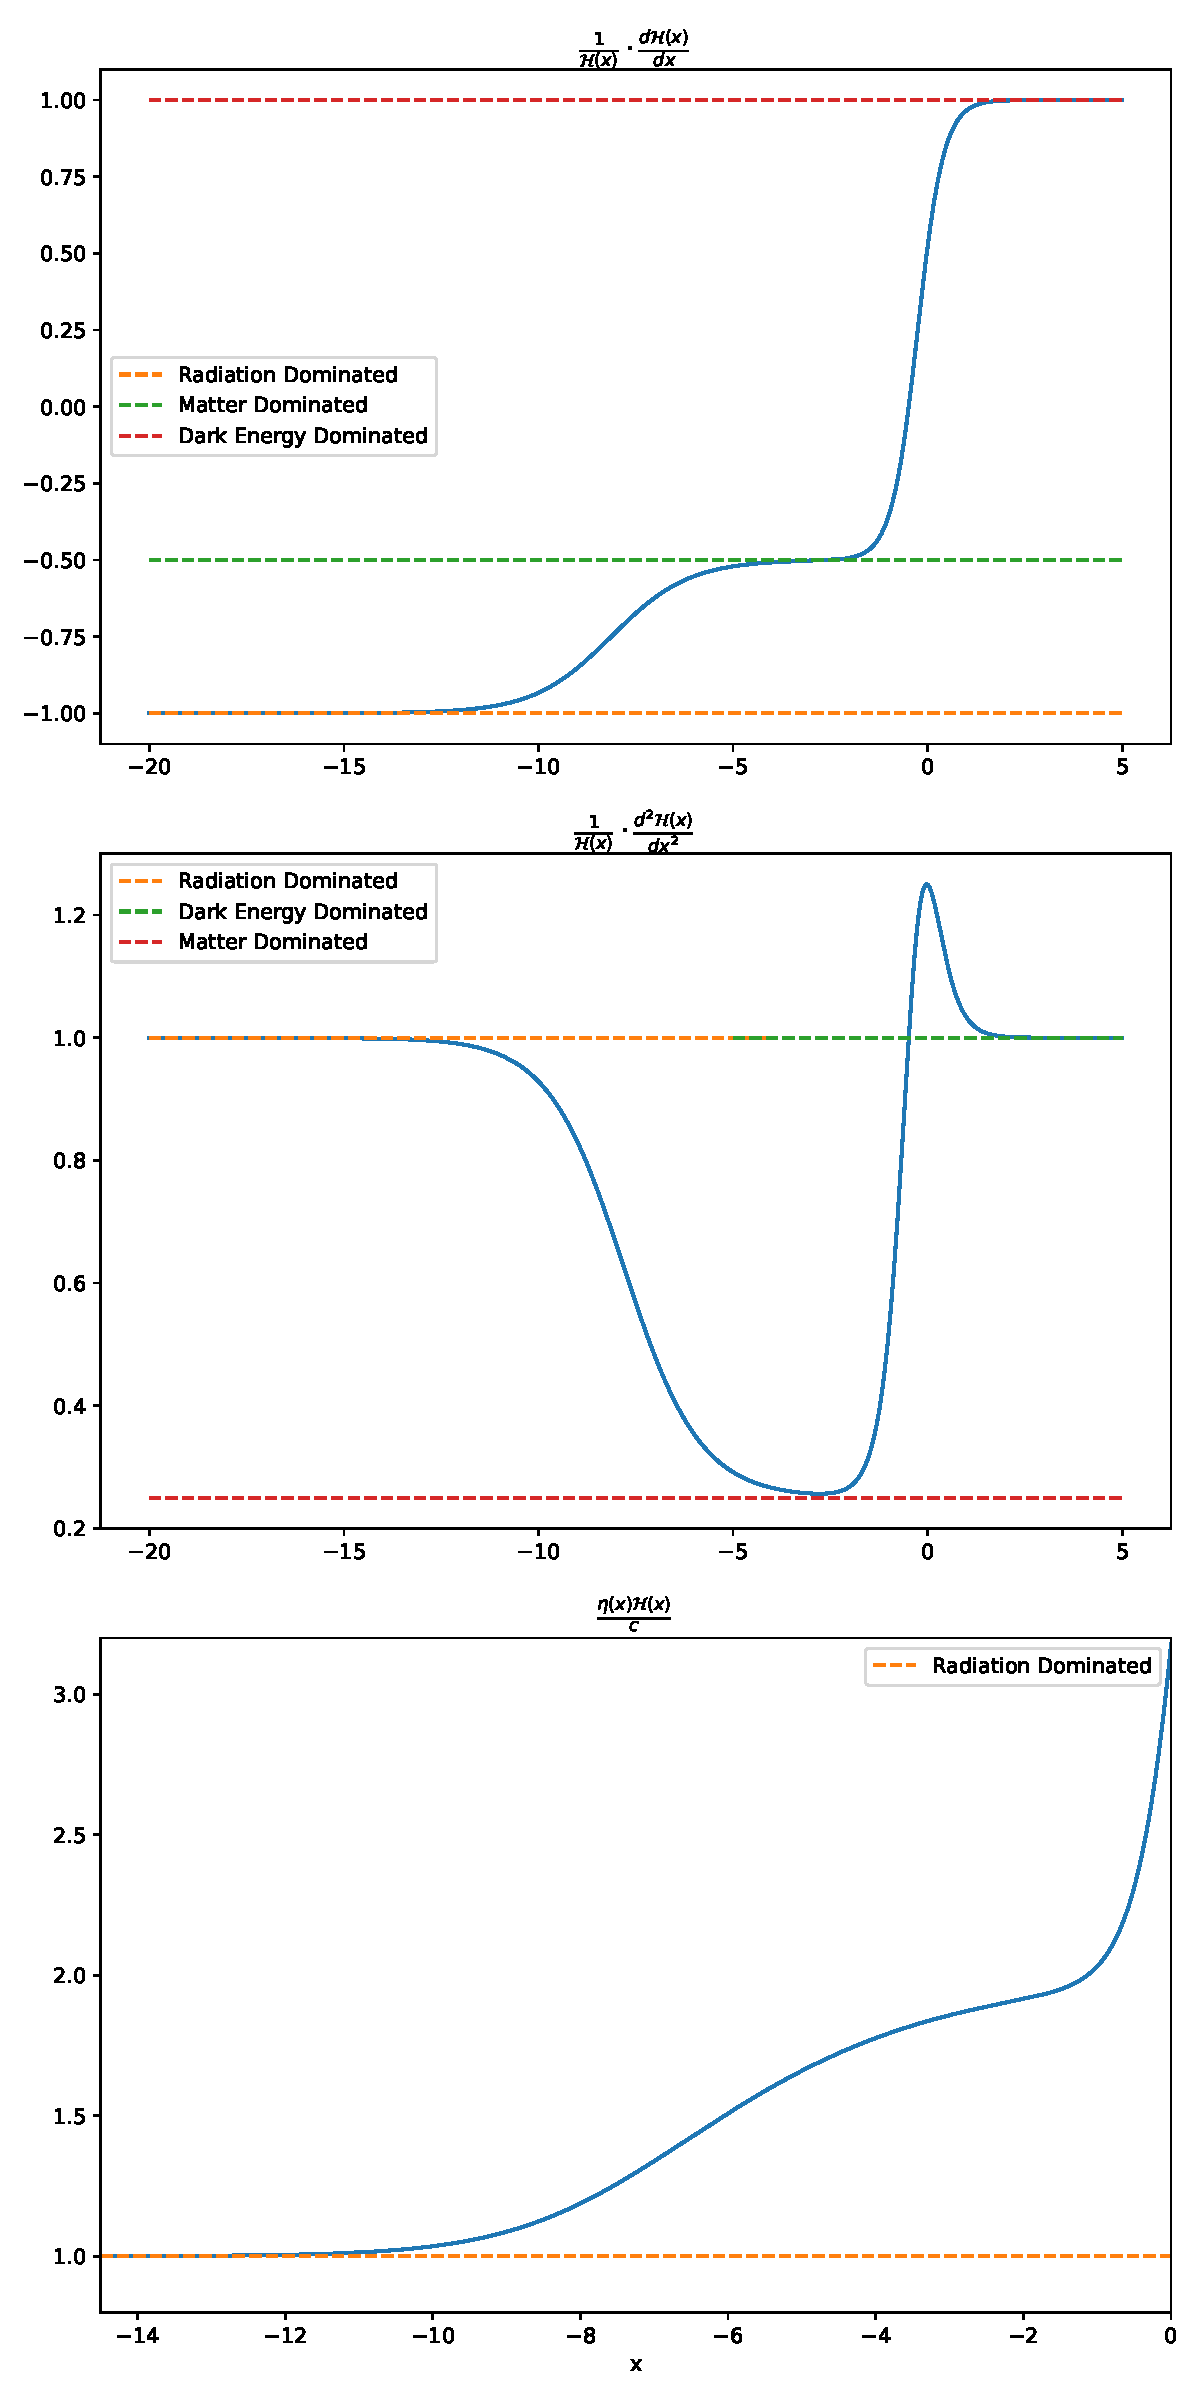
\includegraphics[scale=0.5]{../figures/milestone1/demonstrate_that_code_works.pdf}
   \caption{Plots to demonstrate that the code works properly. The dotted lines are the theoretical predictions.}\label{fig:M1_test_1}

\end{figure}



\subsection{Our results}



In figure \ref{fig:M1_Hp} we show a plot of the conformal Hubble parameter, $\mathcal{H}(x)$, which will often appear in calculations. $\mathcal{H}(x)$ is in actuality just $\dot{a}$, i.e. the rate of which the scale factor changes 
with respect to $x$. For two galaxies following the Hubble flow, the comoving distance, $d_\mathrm{comoving}$, is constant and equal to the physical distance today, since $d = a\cdot d_\mathrm{comoving}$.
The rate of change in the distance between them, $v$, is simply $v = \dot{a}\cdot d_\mathrm{comoving} = \mathcal{H}d_\mathrm{comoving} = Hd$, which is the Hubble law.
Since we study the FLRW universe, we know that massive particles follow the Hubble flow, so $v$ tells us firstly that at any given time, particles will move away from us 
twice as fast if they are twice as far away. Secondly, $\mathcal{H}(x)$ is, at any given time, the constant of proportionality for the first relation. In other words, $\mathcal{H}(x)$
is the expansion rate of the universe. In the plot, we see that this rate was largest at early times. We also see that the slope changes around radiation matter equality and around matter dark energy equality.
This can be understood by solving the Friedmann equation with one energy density component at a time. When dark energy becomes more dominant in the total energy density of the universe, the universe start to expand more rapidly again.
This is because the mass density has become too low for mass to be bound by "gravity". This happens at some time before matter dark energy equality as we can see
in the table \ref{tab:M1_times}.\\
\\
In figure \ref{fig:M1_t_x} we see the cosmic time, which is the time measured by an observer following the Hubble flow, plotted against $x$. The scale factor is proportional to $t^{1/2}$ during radiation domination, and proportional to $t^{2/3}$ during matter domination, \cite{Dodelson:MC}.
This explains why there is a change in the slope around radiation matter equality. As expected, the time today is of order giga years.\\
\\
In figure \ref{fig:M1_eta_x} we see the conformal time, $\eta(x)$. The conformal time, measured in length, is the distance light could have travelled, in comoving coordinates,
since the big bang. Measured in time, $\eta$ is then the amount of time light would have used to travel $\eta$ in length. The conversion factor between time and length is the speed of light.
Since $a=1$ today, $\eta(0)$ is then the size of the observable universe today, since light could have travelled those distances since the big bang. $\eta(x)$ is the comoving distance of causality.
The physical distance of causality at cosmic time, $t$, is then $a(t)\cdot \eta(x(t))$. The conformal time, in time, is larger than the cosmic time since the universe has expanded.
The expansion made all distances larger, and if we freeze the expansion, light would need more than 13.8 billion years to travel across the radius of the observable universe.
From table \ref{tab:M1_times} we see that light would need 46.3 billion years to travel this distance. Again we see that the slope changes around radiation matter equality, which is related to the change in $\mathcal{H}$.
The physical reason for why $\eta$ can change with respect to the cosmic time, is that the scale factor changes with time. If the scale factor is constant, $\eta$ will grow linearly. If the 
universe expands with the speed of light everywhere, $\eta$ will be constant, since light will not move relative to the comoving coordinates.\\
\\
In figure \ref{fig:M1_Omegas} we see how much each energy density parameter contributes to the sum of the energy density parameters. We see that the dark energy component
remains a small part of the total energy density in the universe until recently relative to the age of the universe. In the future, dark energy will be the only relevant density parameter,
so the universe will expand faster in the future compared to today. In the radiation dominated era, the universe was dominated by relativistic particles. As the universe
expanded and cooled down, the particles lost energy, and the energy content was dominated by non-relativistic matter. As the universe continued to expand, the mass density
decreases with the scale factor in all three spatial dimensions, i.e. $\rho \propto \frac{1}{a^3}$. Since the cosmological constant is constant everywhere, the total amount of dark energy
must increase when more space is created. This is observed close to $x=0$ in the plot.\\
\\
In figure \ref{fig:M1_data} we see that our model of the universe predicts a luminosity distance curve that agrees reasonably well with observations. This suggests that the universe is close to being flat.
In figure \ref{fig:M1_constraints} we see the $1\sigma$ and $2\sigma$ constraints from MCMC fits to supernova data in the $\Omega_\Lambda$ vs. $\Omega_M$ plane. 
The average value of the small Hubble parameter was $h= 0.70$ with $1\sigma = 0.0064$. We allowed curvature when fitting the data, and our best fit suggests, with $\chi^2=29.28$, that the curvature density parameter, $\Omega_K$,
is equal to 0.11.  


%by the scale factor, so it will be smaller than $H$ except for today where $a = 1$. Large values of $\mathcal{H}$ tells us that the      



\begin{figure}[H]
   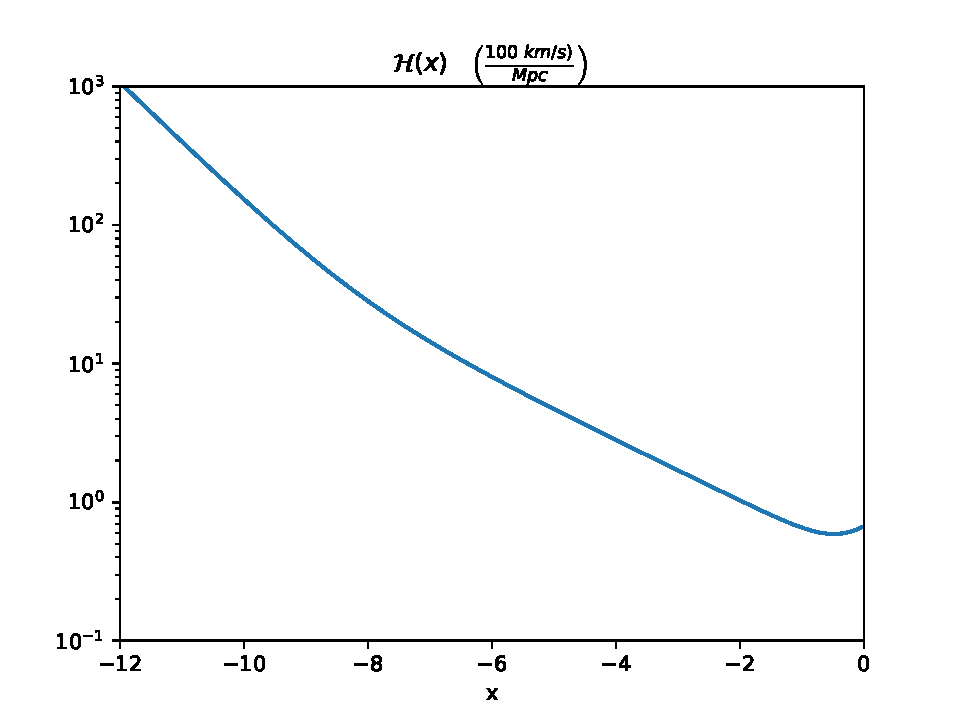
\includegraphics[scale=0.6]{../figures/milestone1/Hp_x.pdf}
   \caption{The conformal Hubble parameter as a function of $x$.}\label{fig:M1_Hp}
\end{figure}

\begin{figure}[H]
   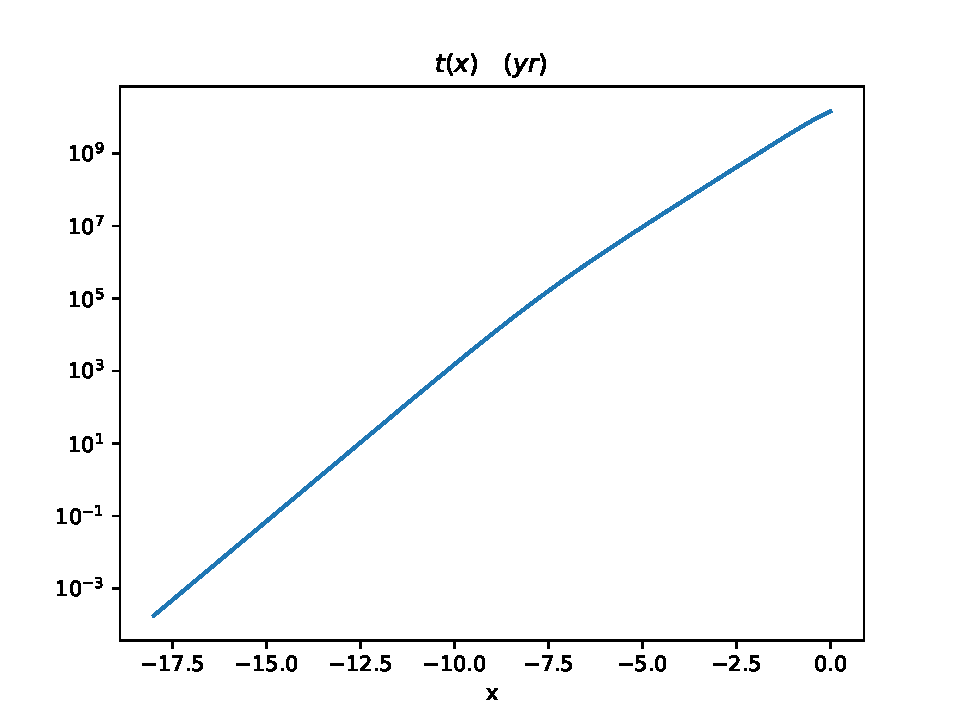
\includegraphics[scale=0.6]{../figures/milestone1/t_x.pdf}
   \caption{The cosmic time as a function of $x$.}\label{fig:M1_t_x}
\end{figure}

\begin{figure}[H]
   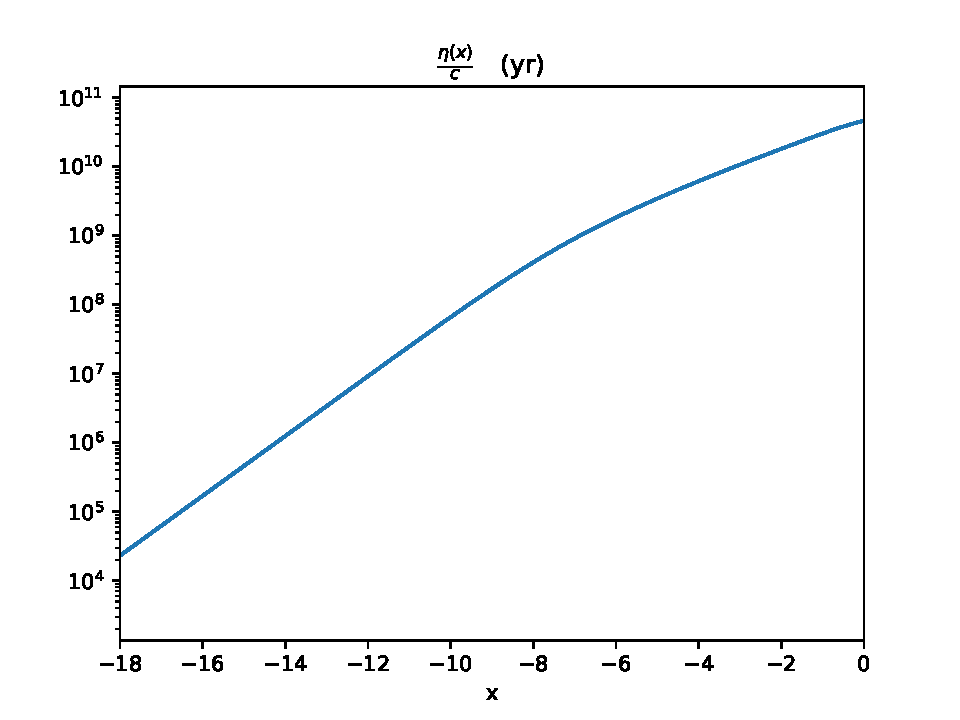
\includegraphics[scale=0.6]{../figures/milestone1/eta_x.pdf}
   \caption{The conformal time as a function of $x$.}\label{fig:M1_eta_x}
\end{figure}

\begin{figure}[H]
   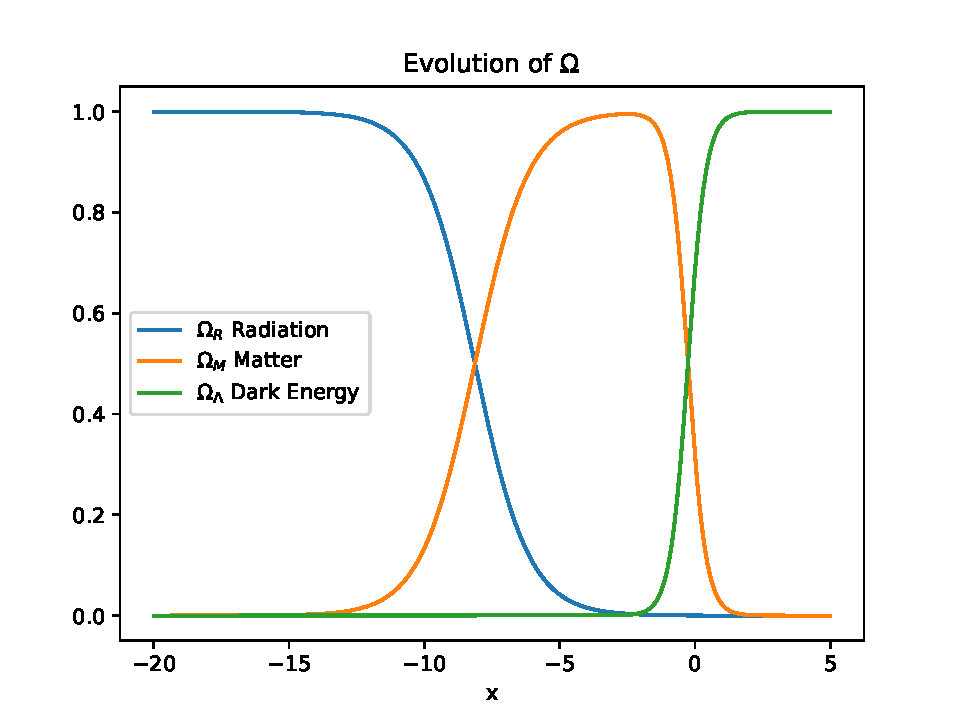
\includegraphics[scale=0.6]{../figures/milestone1/Omegas.pdf}
   \caption{The density parameters as a function of $x$.}\label{fig:M1_Omegas}
\end{figure}

\begin{figure}[H]
   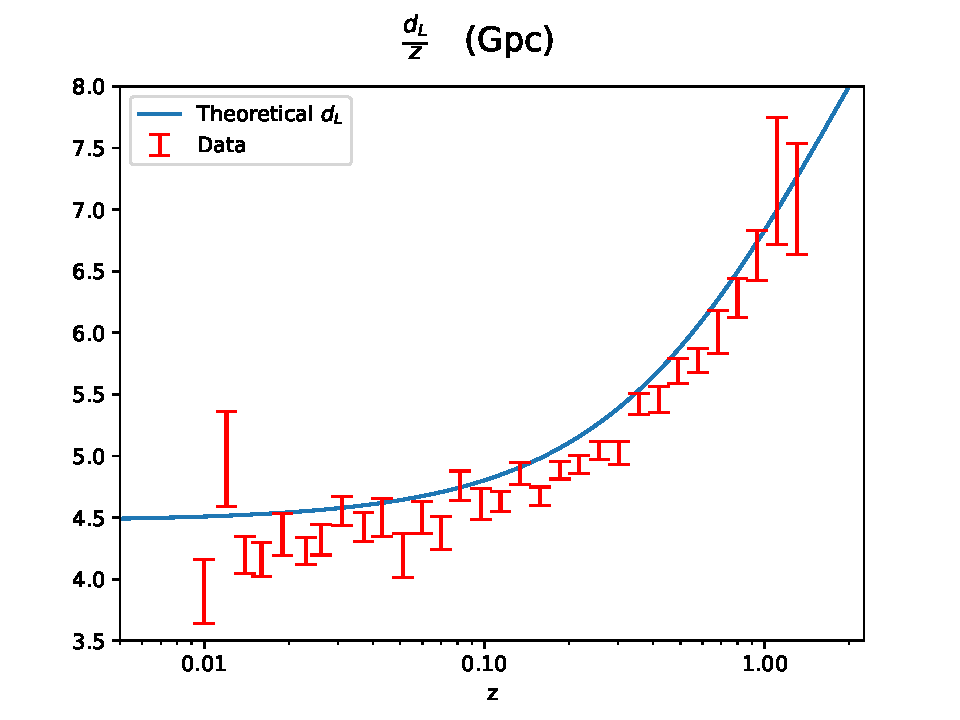
\includegraphics[scale=0.6]{../figures/milestone1/dataplot.pdf}
   \caption{The theoretical luminosity distance, divided by redshift, is plotted against redshift. Actual data from supernova observations is overplotted.}\label{fig:M1_data}
\end{figure}

\begin{figure}[H]
   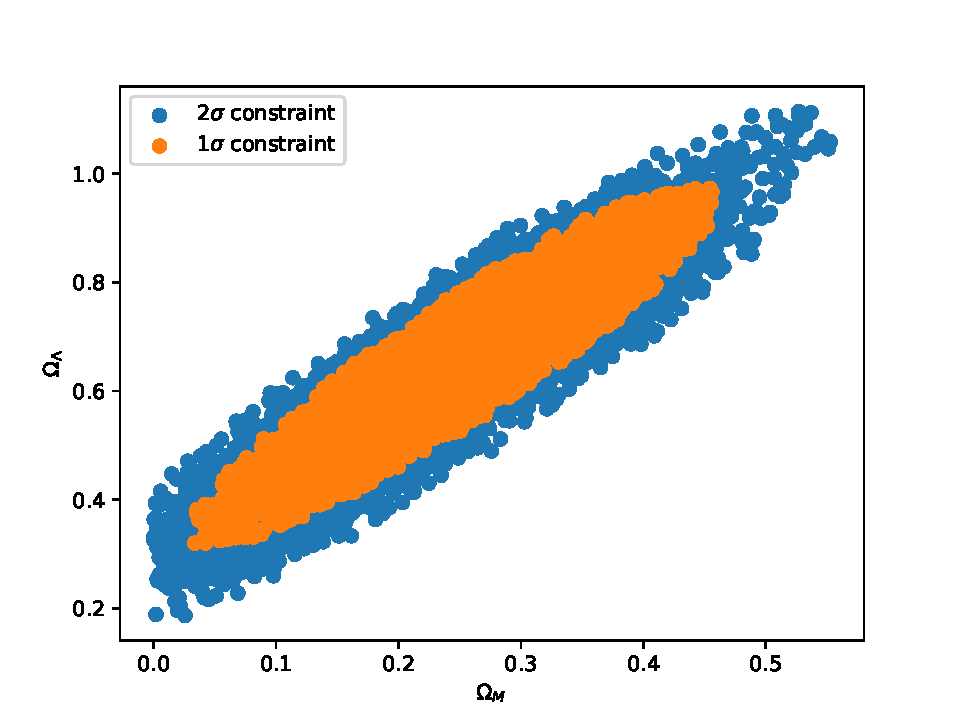
\includegraphics[scale=0.6]{../figures/milestone1/constraints.pdf}
   \caption{The $1\sigma$ and $2\sigma$ constraints from MCMC fits to supernova data in the $\Omega_\Lambda$ vs. $\Omega_M$ plane.}\label{fig:M1_constraints}
\end{figure}

\begin{figure}[H]
   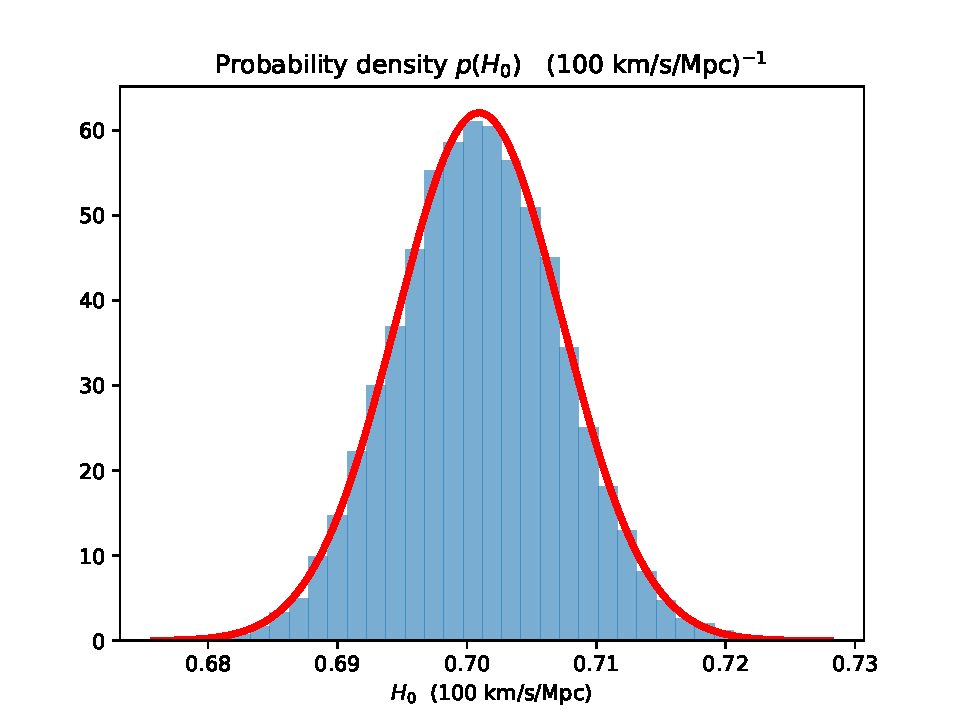
\includegraphics[scale=0.6]{../figures/milestone1/prob_dist_H0.pdf}
   \caption{The probability distribution of the Hubble parameter fitted with a Gaussian.}\label{fig:M1_prob_dist}
\end{figure}

\noindent
\\
In table \ref{tab:M1_times} we show some times for different events in the universe.
\begin{table}[H] %%h! er for å tvinge tabellen til å være nærmest mulig her i dokumentet
   %\begin{center}
     \caption{Important times in cosmology stated in $x$, $z$ and $t$.} %Tabelltekst
     \label{tab:M1_times}
     \begin{tabular}{l|l|r|l} % for hver kolonne har du {a|b|c} der a er for 1.kolonne, b for 2. kolonne etc, l=venstrestil, r=høyrestilt, c = senterstilt. Se posisjonen til tallene i de forskjellige kolonnene. Har du 4 kolonner der alle er senterstilt blir det f.eks. {c|c|c|c}
       \textbf{Event} & \textbf{x, z, t}\\ %innhold i hver kolonne, legg til flere her hvis du har flere kolonner
       %(i) & (m) & (m/s)\\ %enheter for hver kolonne
       \hline %en horisontall linje for å skille overskriften fra tallene under. Vil du ha en slik linje mellom hver rad i tabellen så legg til en \hline mellom hver rad nedover her. Merk \\ er som vanlig linjeskift mens & skiller kolonner
       Radiation-Matter equality & -8.13,  3400.33, 51.06 [$10^3$ yr] \\
       Matter-Dark energy equality & -0.26, 0.29, 10.38 [Gyr]        \\
       Time of cosmic acceleration & -0.49, 0.63, 7.76 [Gyr]\\
       Age of the universe today & 0.00, 0.00, 13.86 [Gyr]  \\
       Conformal time today  & 1.90, -0.85, 46.32 [Gyr]\\

       %$Y_\mathrm{p}$ & 0\\
       \hline
     \end{tabular}
   %\end{center}
 \end{table}



\section{Milestone II}
%Some introduction about what it is all about.
%Calculated the optical depth and the visibility function, which is important for the intensity of the CMB photons.
When the photon temperature in the universe became too low for photons to ionize the hydrogen atom, a period of recombination begun in the universe. In this period, neutral hydrogen
started to form, and the free electron density decreased. This led to a dramatic change in the scattering rate of light, since photons scatter on free electrons. After this period, light could travel mostly freely towards us. These 
photons are the CMB photons that we in the end wish to study.\\
\\  
The aim of this milestone is to calculate the optical depth for photons emitted at time $x$ observed by us today, and the visibility function. More details on these functions later. 

\subsection{Theory}

The photon intensity can decrease when photons travel through a medium. This can be due to Thomson scattering, where photons interact with free electrons and the direction
of propagation changes. For an initial intensity $I_0$, the resulting intensity at any given displacement from the origin, $y$, inside the medium can be described by
\begin{equation}
   I(y) = I_0e^{-\tau(y)},
\end{equation}   
where $\tau(y)$ is the optical depth as a function of $y$. Since intensity is a conserved quantity if light travels unimpeded,
the optical depth can tell us how much of the initial intensity that has been lost due to processes in the medium, e.g. scattering. $\tau$ is defined by
\begin{equation}
   \tau(\eta) = \int_{\eta}^{\eta_0} n_e(\eta') \sigma_T a(\eta') d\eta',
\end{equation}
where $n_e$ is the free electron density and $\sigma_T$ is the Thomson cross-section. The optical depth is here defined as a function of conformal time, 
such that $\tau(\eta)$ is related to the fraction of the intensity that remains today over the initial intensity at $\eta$. The differential equation for $\tau$ as a function
of our time variable $x$ is 
\begin{equation}
   \tau' = \frac{d\tau}{dx} = -\frac{c n_e \sigma_T }{H}.
\end{equation} 

We define the free electron fraction as
\begin{equation}
X_e =  n_e/n_H,
\end{equation}
where $n_H$ is the proton density. We assume no heavier elements. Using that the mass of a proton is approximately equal to the mass of hydrogen, $m_H$
we get \begin{equation}
   n_H = \frac{\Omega_{b0} \rho_{c0}}{m_H a^3}.
\end{equation}
$X_e$ can be solved in two different regimes. The first regime is when everything is in equilibrium, and the second regime is when the free electron fraction starts to decrease.
The first regime is governed by the Saha equation given by
\begin{equation}
   \frac{X_e^2}{1-X_e} = \frac{1}{n_b} \left(\frac{m_e
T_b}{2\pi}\right)^{3/2} e^{-\epsilon_0/T_b},
\end{equation}
where $n_b = n_H$, $m_e$ is the electron mass, $T_b$ is the baryon temperature and $\epsilon_0$ is the ionization energy of hydrogen. Since the Saha equation hold when 
photons and baryons are in equilibrium, the baryon temperature is equal to the photon temperature, $T_{CMB}/a$. The second regime is governed by the Peebles equation given below
\begin{equation}
   \frac{dX_e}{dx} = \frac{C_r(T_b)}{H} \left[\beta(T_b)(1-X_e) - n_H
\alpha^{(2)}(T_b)X_e^2\right],
\end{equation}
where 
$$
\boxed{
\begin{aligned}
C_r(T_b) &= \frac{\Lambda_{2s\rightarrow1s} + \Lambda_{\alpha}}{\Lambda_{2s\rightarrow1s} + \Lambda_{\alpha} + \beta^{(2)}(T_b)}, \,\,{\rm (dimensionless)},\\
H &,  \,\,{\rm (dimension~1/s)}\\
\Lambda_{2s\rightarrow1s} &= 8.227 \textrm{s}^{-1}, \,\,{\rm (dimension~1/s)}\\
\Lambda_{\alpha} &= H\frac{(3\epsilon_0)^3}{(8\pi)^2 n_{1s}}, \,\,{\rm (dimension~1/s)}\\
n_{1s} &= (1-X_e)n_H, \,\,{\rm (dimension~1/m^3)}\\
n_H &= (1-Y_p)\frac{3H_0^2\Omega_{b0}}{8\pi G m_H a^3}, \,\,{\rm (dimension~1/m^3)}\\
\beta^{(2)}(T_b) &= \beta(T_b) e^{3\epsilon_0/4T_b}, \,\,{\rm (dimension~1/s)}\\
\beta(T_b) &= \alpha^{(2)}(T_b) \left(\frac{m_eT_b}{2\pi}\right)^{3/2} e^{-\epsilon_0/T_b}, \,\,{\rm (dimension~1/s)} \\
\alpha^{(2)}(T_b) &= \frac{64\pi}{\sqrt{27\pi}}\frac{\alpha^2}{m_e^2}\sqrt{\frac{\epsilon_0}{T_b}}\phi_2(T_b), \,\,{\rm (dimension~m^3/s)}\\
\phi_2(T_b) &= 0.448\ln(\epsilon_0/T_b), \,\,{\rm (dimensionless)}.
\end{aligned}
}
$$
where $\alpha \simeq \frac{1}{137.0359992}$. We now take transition rates between the 1s and 2s quantum states of the hydrogen atom.\\
\\
The visibility function is given by $\tilde{g}(x) = -\tau'e^{-\tau}$. \\
\\
Finally, the sound horizon is given by 
$$\boxed{\begin{aligned}   
   s(x) &= \int_0^{a} \frac{c_s dt}{a} = \int_{-\infty}^{x} \frac{c_s dx}{\mathcal{H}} \to \frac{ds(x)}{dx}
 = \frac{c_s}{\mathcal{H}}\\
 &\text{with}\,\,\,s(x_{\rm ini}) = \frac{c_s(x_{\rm ini})}{\mathcal{H}(x_{\rm ini})}     
\end{aligned}}$$ 
 where $c_s = c \sqrt{\frac{R}{3(1+R)}}$ where $R = \frac{4\Omega_{\gamma 0}}{3\Omega_{b 0} a}$.

\subsection{Implementation details}
The code needs the background solution found in the previous milestone in order to run. The code solves the Saha and Peebles equations and calculates the optical depth and the visibility function.
The differential equations are solved with a Runge-Kutta 4 ODE solver, and the result is splines using a cubic spline.
We solve the quantities of interest from $x=-20$ until $x=0$. We solve for 1000 points linearly spaced. 
We switch from the Saha equation to the Peebles equation when $X_e$ reaches 0.99.



\subsection{Results}
\subsubsection{Testing the code.}
The code was mainly tested by comparing our plots to the plots of \cite{winther:2023} and \cite{Callin}.

\subsubsection{Our results}
In figure \ref{fig:M2:X_e} we see how the free electron fraction, $X_e$, evolves with time $x$. The blue plot is the free electron fraction using a combination of both
the Saha and the Peebles equations. We see that before recombination, there were equally many free electrons as there were protons. Around recombination, we see 
that $X_e$ has dropped to a tenth of its initial value, such that there are 10 times fewer free electrons at this time, using that the comoving proton density is constant. We aslo see
that $X_e$ seems to stabilize before it reaches $10^{-4}$. The Saha prediction is plotted in orange. We see that the Saha equation predicts that $X_e$ decreases more rapidly, and does not 
stabilize, but goes to zero. We see from the dotted line that recombination happens after $X_e$ has started to decrease, which is consistent with intuition, as there must be fewer free electrons after atoms have started to form.
The time of recombination was calculated using the visibility function, which
we will discuss later.\\
\\
In figure \ref{fig:M2:taus} we see the optical depth for photons emitted at time $x$ received by us today. Since the optical depth tells us how the intensity of light decreases as it travels through a medium,
we expect $\tau$ in general to be larger for larger $x$ values as light has travelled a longer distance. We also expect $\tau$ to be larger if $X_e$ is closer to one, since light scatters off free electrons. We clearly see that the optical depth is very large for photons that were 
emitted before recombination. After recombination, the universe became transparent. This is seen in the plot, as $\tau$ is several orders of magnitude lower after recombination, which
means that photons emitted after recombination travelled mostly unimpeded. The reason why the optical depth decreases with $x$ before recombination when $X_e$ is constant is because light
travels a shorter distance through the medium when $x$ decreases. $\tau$ is obviously zero at $x=0$ since there is no time for light to be scattered from $x=0$ to $x=0$. We see that $\tau$ is of order $10^4$ at x=-12.
This means that the observed intensity for light emitted at $x=-12$ is approximately a factor $10^{-4343}$ smaller than the initial intensity. Therefore, it is not possible,
in a practical sense at least, to detect photons that were emitted before recombination.\\ 
\\
  
\begin{figure}[H]
   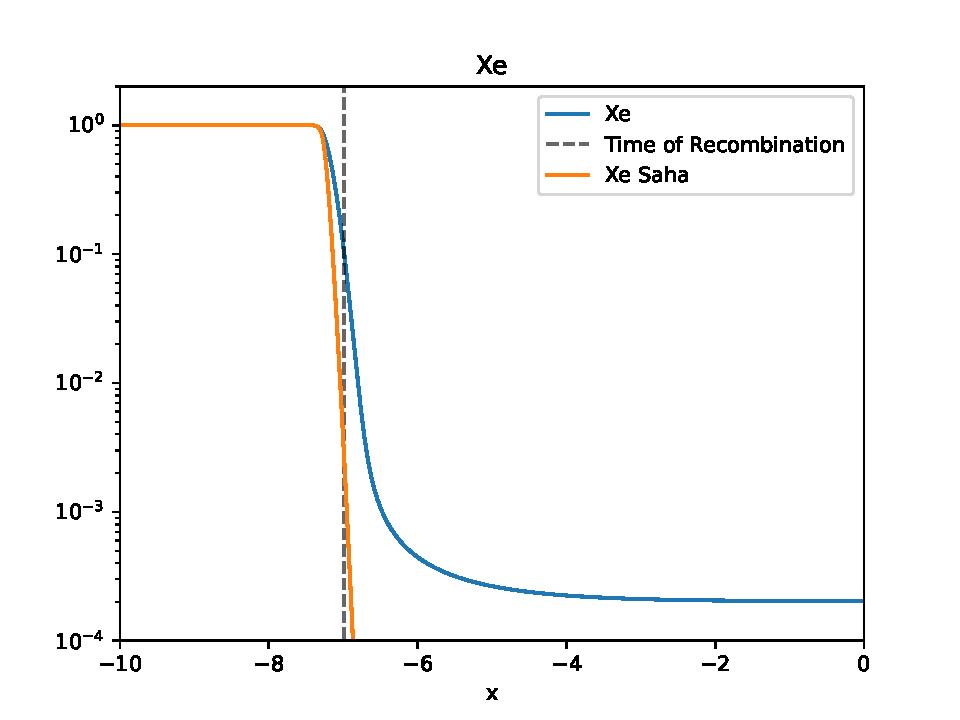
\includegraphics[scale=0.5]{../figures/milestone2/X_e.pdf}
   \caption{The free electron fraction, $X_e$, plotted against $x$. The Saha prediction is also included in orange.}\label{fig:M2:X_e}
\end{figure}

\begin{figure}[H]
   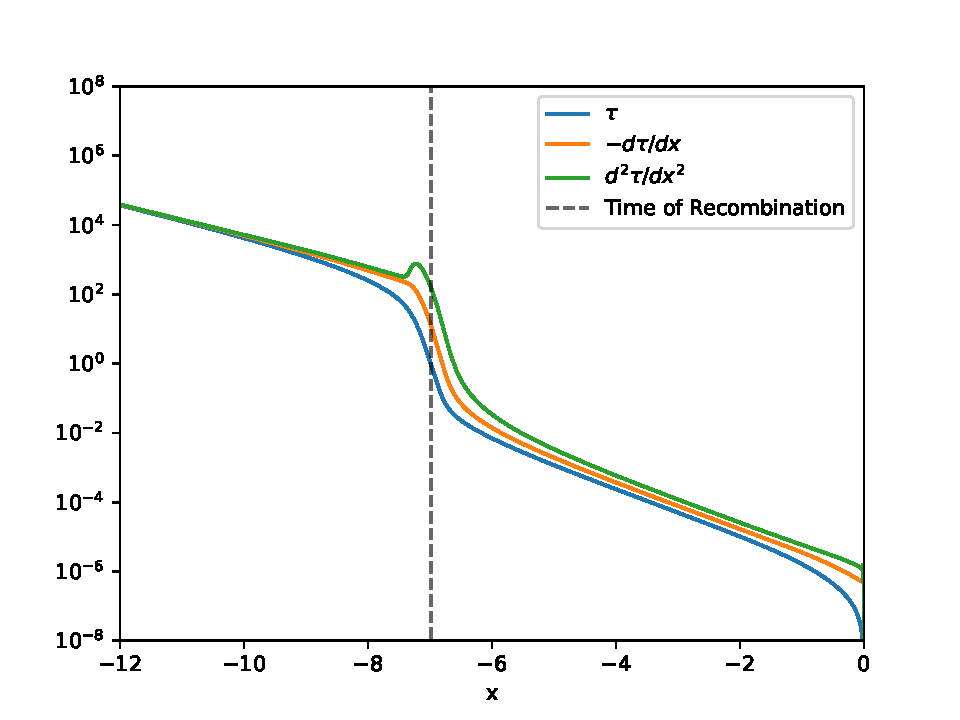
\includegraphics[scale=0.5]{../figures/milestone2/taus.pdf}
   \caption{The optical depth with its first and second derivatives are plotted against $x$.}\label{fig:M2:taus}
\end{figure}

\begin{figure}[H]
   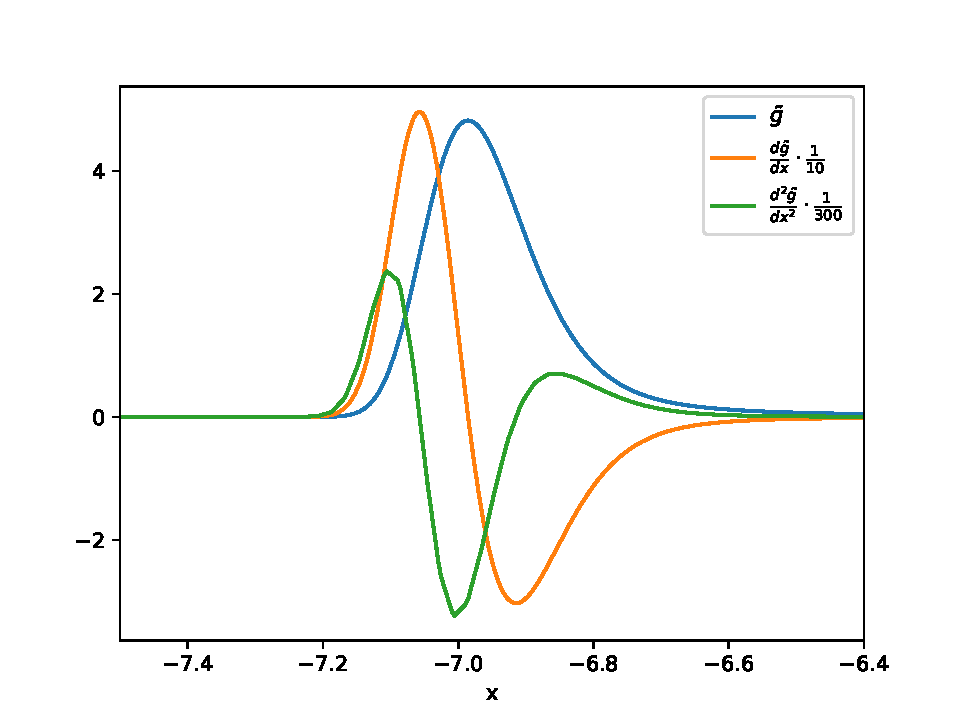
\includegraphics[scale=0.5]{../figures/milestone2/g_tilde_plots.pdf}
   \caption{The visibility function with its first and second derivatives are plotted against $x$.}\label{fig:M2:g_tilde_plots}
\end{figure}

\noindent
In figure \ref{fig:M2:g_tilde_plots} we see the visibility function.
Since the visibility function tells us the probability density that a photon scattered for the last time at $x$, the peak in the visibility function tells us the time 
when a photon was most likely to have scattered for the last time. By defining the last scattering surface to happen at this time, we get a value of $x=-6.98$ for the last scattering surface. The corresponding 
redshift is $z = 1079.73$ with cosmic time $t=378004$ years. Recombination is the time when free electrons combined with protons to form hydrogen. This was possible
since the photon temperature was, in general, too low to free the electrons by ionizing the hydrogen atoms. Recombination can therefore be defined when the abundance of 
free electrons reached a threshold value. We choose recombination to happen when the free electron fraction takes the value of 0.1. Doing this we get exactly the same
value of $x$ as we did for the time of the last scattering surface. This reason why the values are exactly the same could be related to the splines, or to the
resolution in $x$ not being precise enough when extracting information from the arrays. Either way, this suggests that recombination happens very close to the last scattering
surface. Knowing this, we can use the prediction of $X_e$ from the Saha equation to give an estimate of both when recombination and the last scattering surface happened according to the Saha equation.
Using $X_e=0.1$ in the Saha equation we get that recombination happened at $x= -7.14$, $z = 1260$, $t=290354$ years.
From figure \ref{fig:M2:X_e} we see that the Saha equation predicts that the free electron fraction drops more rapidly than the Peebles eqaution predicts. Recombination will therefore happen earlier
using the Saha equation.\\
\\
The free electron density today is $2\cdot 10^{-4}$ meaning that for every two free electrons in the universe today, there are ten thousand protons. Since the comoving 
number density of protons is constant, we see that the free electron fraction can be rewritten into $\frac{{n_e}_\mathrm{today}}{{n_e}_\mathrm{initial}} = 2\cdot 10^{-4}$, such that free electrons 
are five thousand times rarer today as they were initially, i.e. before recombination.\\
\\
The sound horizon is the distance sound could have travelled in the proton-electron-photon plasma from the Big Bang until recombination, where the plasma ceases to exist.
Since primordial energy density contrasts created sound waves in the plasma, and these sound waves froze as the plasma became neutral, we can expect to see those sound 
waves in the universe today. The sound horizon at recombination was 0.145 Gpc in comoving coordinates, i.e. in FLRW coordinates. To get the physical distance at any given time, we
can multiply by the value of the scale factor at that time. Since we are only interested in physical distances today, we multiply by $a_0 =1$, such that the physical distance
of the sound horizon, at recombination, measured today is 0.145 Gpc. We therefore expect 0.145 Gpc to be the largest distances where the CMB is in equilibrium,
since heat could not travel further than those distances. Therefore, people were surprised when CMB photons from the opposite sides of the universe appeared to be very close to equilibrium. This problem was solved by inflation.  




\section{Milestone III}
%husk a snakke om at vi løser fra radiation domination, men initial betingelsene er fra inflasjon p.g.a. horizon frys...
%sound hoizon vs. particle horizon
%Some introduction about what it is all about.
%In this milestone we look at 
In this milestone we calculate the evolution of the structures in the universe from after inflation until today.  In practice, this is done by 
solving the perturbed Einstein-Boltzmann equations numerically with initial conditions from inflation. This will give us the time evolution of the different physical quantities we are interested
in at different Fourier scales, $k$. We will go into more detail in the theory section. A detailed derivation of the relevant equations is given in \cite{winther:2023}. \\
\\
The observed CMB is a measurement of the photon temperature field today. In order to reconstruct the statistical properties of the observations, we need
to know how the structures in the universe evolved from some initial state to the state we observe today. This is important as matter perturbations will source gravitational
wells that, by relativistic effects, will redshift the photons originating from inside the well. This will directly increase the photon temperature fluctuations that we are interested in.   

\subsection{Theory}
%The theory behind this milestone.
%Boltzmann equations, spherical harmonics, perturbation theory...
Some regions in the early universe expanded more rapidly than others during inflation due to quantum fluctuations in the inflaton field, \cite{winther:2023}. These fluctuations
made the energy density of the universe inhomogeneous, which introduced fluctuations in the famous Friedmann-Lemaître-Robertson-Walker (FLRW) metric. We can find the initial conditions for the metric perturbations, $\Psi$ and $\Phi$, in the Newtonian gauge, and from there find the initial conditions for
the energy density perturbations of interest. This is done in \cite{winther:2023}.\\
\noindent
\\
The perturbations in the photon temperature field, $\delta T$, today are much smaller than the background temperature, $\overline{T}$. The same is true for the matter field on large scales.
This suggests that we can apply linear perturbation theory on the distribution functions and expect 
that the result will be valid today. The perturbed distribution functions, $f_i$, for baryons, photons and CDM take the form \[f_i(t,\vec{x},\vec{p})
 = \overline{f_i}(t,\vec{p}) + \delta f_i(t,\vec{x},\vec{p}),\] where $\overline{f_i}$ is the background distribution function and $\delta f_i$ is the perturbation. These perturbations will of course perturb the 
energy momentum tensor in the Einstein equations, which in turn will perturb the metric. This will then change how particles move through space and time, \cite{winther:2023}. We will therefore have a system of coupled differential equations.
The perturbed Einstein-Boltzmann equations can be solved in Fourier space with $x = \ln a$ as the time variable. The photon temperature perturbations, here defined as the relative perturbation $\Theta = \delta T/\overline{T}$, are expanded in Legendre multipoles,
such that we are left with multipoles, $\Theta_\ell$ of the photon distribution. Similarly, the CDM and baryon overdensities we solve for are defined as $\delta_\mathrm{CDM} = \frac{\delta \rho_{CDM}}{\overline{\rho}_{CDM}}$ and $\delta_\mathrm{b} = \frac{\delta \rho_{b}}{\overline{\rho}_{b}}$.
The velocities are defined similarly, such that they are dimensionless. We do not solve the equations for polarization, and neutrino perturbations are not included.\\ 
\\
The initial conditions:
$$
\boxed{
\begin{aligned}
\Psi &= -\frac{2}{3} \\
\Phi &= -\Psi \\
\delta_{\rm CDM} &= \delta_b = -\frac{3}{2} \Psi \\
v_{\rm CDM} &= v_b = -\frac{ck}{2\mathcal{H}} \Psi \\
&\text{Photons:}\\
\Theta_0 &= -\frac{1}{2} \Psi \\
\Theta_1 &= +\frac{ck}{6\mathcal{H}}\Psi \\
\Theta_2 &= -\frac{20ck}{45\mathcal{H}\tau^\prime} \Theta_1 \\
\Theta_\ell &= -\frac{\ell}{2\ell+1} \frac{ck}{\mathcal{H}\tau^\prime} \Theta_{\ell-1}\\
\end{aligned}
}
$$

The photon equations:
$$
\boxed{
\begin{aligned}
\Theta^\prime_0 &= -\frac{ck}{\mathcal{H}} \Theta_1 - \Phi^\prime, \\
\Theta^\prime_1 &=  \frac{ck}{3\mathcal{H}} \Theta_0 - \frac{2ck}{3\mathcal{H}}\Theta_2 +
\frac{ck}{3\mathcal{H}}\Psi + \tau^\prime\left[\Theta_1 + \frac{1}{3}v_b\right], \\
\Theta^\prime_\ell &= \frac{\ell ck}{(2\ell+1)\mathcal{H}}\Theta_{\ell-1} - \frac{(\ell+1)ck}{(2\ell+1)\mathcal{H}}
\Theta_{\ell+1} + \tau^\prime\left[\Theta_\ell - \frac{1}{10}\Theta_2
\delta_{\ell,2}\right],\\ 
& \mathrm{where} \ \ 2 \leq \ell \textless \ell_{\textrm{max}} \\
\Theta_{\ell}^\prime &= \frac{ck}{\mathcal{H}}
\Theta_{\ell-1}-c\frac{\ell+1}{\mathcal{H}\eta(x)}\Theta_\ell+\tau^\prime\Theta_\ell,
\quad\quad \ell = \ell_{\textrm{max}}\\
\end{aligned}
}
$$

Cold dark matter and baryons:
$$
\boxed{
\begin{aligned}
\delta_{\rm CDM}^\prime &= \frac{ck}{\mathcal{H}} v_{\rm CDM} - 3\Phi^\prime \\
v_{\rm CDM}^\prime &= -v_{\rm CDM} -\frac{ck}{\mathcal{H}} \Psi \\
\delta_b^\prime &= \frac{ck}{\mathcal{H}}v_b -3\Phi^\prime \\
v_b^\prime &= -v_b - \frac{ck}{\mathcal{H}}\Psi + \tau^\prime R(3\Theta_1 + v_b) \\
\end{aligned}
}
$$
Metric perturbations:
$$
\boxed{
\begin{aligned}
\Phi^\prime &= \Psi - \frac{c^2k^2}{3\mathcal{H}^2} \Phi\\
&+ \frac{H_0^2}{2\mathcal{H}^2}
\left[\Omega_{\rm CDM 0} a^{-1} \delta_{\rm CDM} + \Omega_{b 0} a^{-1} \delta_b + 4\Omega_{\gamma 0}
a^{-2}\Theta_0\right] \\
\Psi &= -\Phi - \frac{12H_0^2}{c^2k^2a^2}\left[\Omega_{\gamma 0}\Theta_2\right], \\
\end{aligned}
}
$$
where $R = \frac{4\Omega_{\gamma 0}}{3\Omega_{b 0} a}$. Some of these equations are numerically unstable early on, where the large value of $\tau^\prime$ is multiplied by the small value of $(3\Theta_1+v_b)$.  
This regime is known as the tight coupling regime, where the universe was opaque, and it can be related to time when the following three conditions hold simultaneously: $|\tau^\prime|>10$, $|\tau^\prime|>10\cdot \frac{ck}{\mathcal{H}}$ and
$x\leq -8.3$. The unstable equations are rewritten below.

$$
\boxed{
\begin{aligned}
q &= \frac{-[(1-R)\tau^\prime + (1+R)\tau^{\prime\prime}](3\Theta_1+v_b)}{(1+R)\tau^\prime + \frac{\mathcal{H}^\prime}{\mathcal{H}} -1}\\
  &\frac{-\frac{ck}{\mathcal{H}}\Psi + (1-\frac{\mathcal{H}^\prime}{\mathcal{H}})\frac{ck}{\mathcal{H}}(-\Theta_0 +
2\Theta_2) - \frac{ck}{\mathcal{H}}\Theta_0^\prime}{(1+R)\tau^\prime + \frac{\mathcal{H}^\prime}{\mathcal{H}} -1}\\
v_b^\prime &= \frac{1}{1+R} \left[-v_b - \frac{ck}{\mathcal{H}}\Psi + R(q +
\frac{ck}{\mathcal{H}}(-\Theta_0 + 2\Theta_2) - \frac{ck}{\mathcal{H}}\Psi)\right]\\
\Theta^\prime_1 &= \frac{1}{3} (q - v_b^\prime).
\end{aligned}
}
$$
The $2 \leq l$ photon multipoles in the tight coupling regime are given by the same expressions as in the initial conditions, but these multipoles are very small in this regime,
so we can simply set them to zero, but we choose to calculate the $\Theta_2$ multipole for higher accuracy.\\
\\

 


\subsection{Implementation details}
We solved the differential equations in two different regimes and "sewed" the solutions together.
Since the last value in the first regime was used as an initial condition for the second regime, we removed the last value 
in the first regime, when "sewing" the solutions together, to remove the overlap between the solutions. A for loop was used to loop through all the Fourier scales, $k$, of interest.
The differential equations were solved using a Runge-Kutta 4 ODE solver. The solution was then splined with a 2D spline, since we have a complete solution in time for each $k$ value.\\ \\
Solutions of the background universe and the recombination history of the universe was also used. We solved the system from x=-20 to x=0 with 1000 linearly spaced points.
The $k/Mpc$ values range from $5\cdot 10^{-5}$ to 0.3 with 100 logarithmically spaced points.

\subsection{Results}

\subsubsection{Test results}
The code produces the following results with the cosmological test parameters given in table \ref{tab:test_parameters}. All the figures show plots at three different scales.
In figures \ref{fig:test1} and \ref{fig:test2} we see the density perturbation and the velocity, respectively, for both CDM and baryons. In figures \ref{fig:test3}
and \ref{fig:test4} we see the photon temperature monopole, $\Theta_0$, and the photon temperature dipole, $\Theta_1$, respectively. The gravitational potential, $\Phi$, is plotted
in figure \ref{fig:test5}. All plots seem to agree with the plots shown in \cite{winther:2023}.   


\begin{table}[h!] %%h! er for å tvinge tabellen til å være nærmest mulig her i dokumentet
   %\begin{center}
     \caption{Cosmological test parameters.} %Tabelltekst
     \label{tab:test_parameters}
     \begin{tabular}{l|l}%|r} % for hver kolonne har du {a|b|c} der a er for 1.kolonne, b for 2. kolonne etc, l=venstrestil, r=høyrestilt, c = senterstilt. Se posisjonen til tallene i de forskjellige kolonnene. Har du 4 kolonner der alle er senterstilt blir det f.eks. {c|c|c|c}
       \textbf{Parameter} & \textbf{Value}\\% & \textbf{Unit}\\ %innhold i hver kolonne, legg til flere her hvis du har flere kolonner
       %(i) & (m) & (m/s)\\ %enheter for hver kolonne
       \hline %en horisontall linje for å skille overskriften fra tallene under. Vil du ha en slik linje mellom hver rad i tabellen så legg til en \hline mellom hver rad nedover her. Merk \\ er som vanlig linjeskift mens & skiller kolonner
       $h$ & 0.7\\
       $\Omega_\mathrm{b}$ & 0.05\\
       $\Omega_\mathrm{CDM}$& 0.45\\
       $\Omega_\mathrm{\Lambda}$ & 0.5\\
       $\Omega_\mathrm{k}  $     & 0\\
       $\Omega_\mathrm{\nu}$ & 0\\
       $T_\mathrm{CMB}$ & 2.7255 $[K]$\\
       %$Y_\mathrm{p}$ & 0\\
       \hline
     \end{tabular}
   %\end{center}
 \end{table}

\begin{figure}[h!]
   %\hspace{-0.48cm}   
   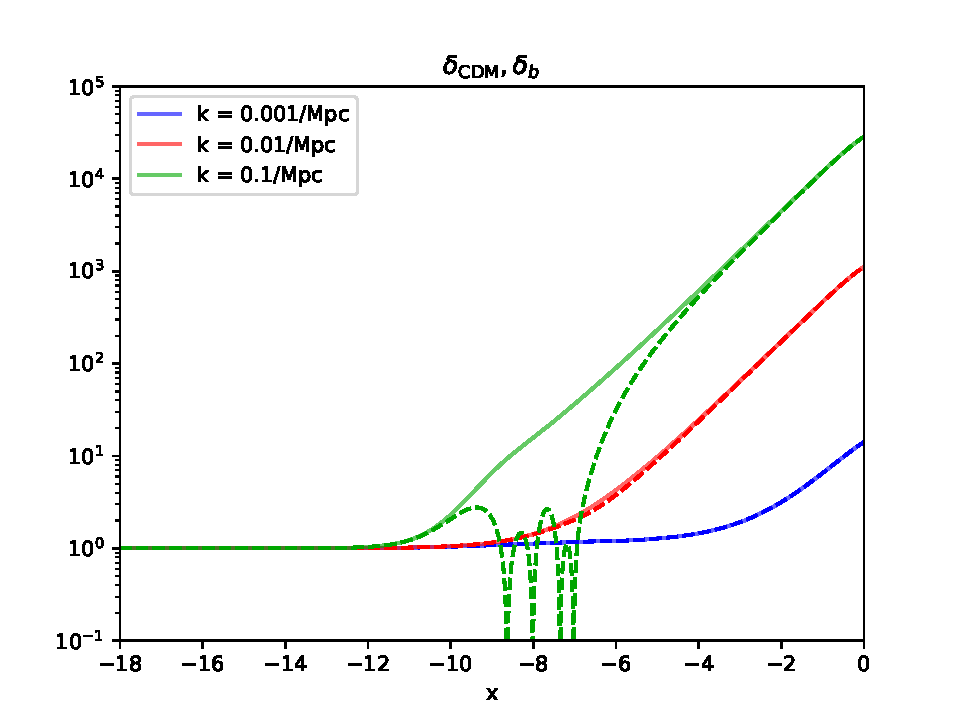
\includegraphics[scale=0.6]{../figures/milestone3/test_delta_cdm_delta_b.pdf}
   \caption{The CDM overdensity, in solid lines, and the absolute value of the baryon overdensity,
    in dotted lines, are plotted at different scales, $k$.}\label{fig:test1}
\end{figure}

\begin{figure}[h!]
   %\hspace{-0.48cm}   
   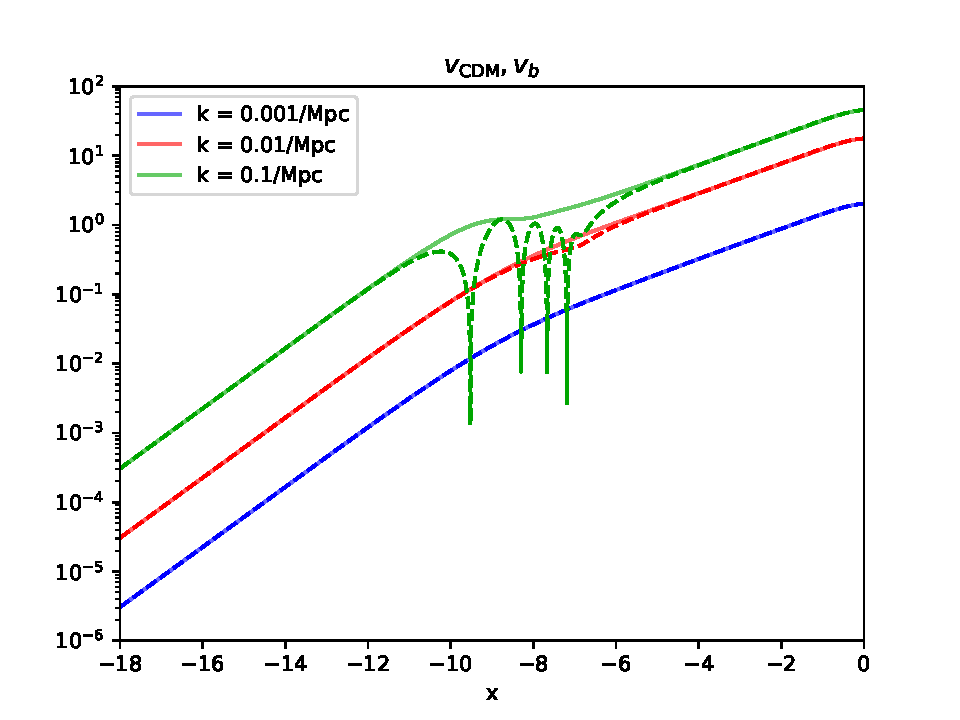
\includegraphics[scale=0.6]{../figures/milestone3/test_v_cdm_v_b.pdf}
   \caption{The CDM velocities, in solid lines, and the absolute value of the baryon velocities,
    in dotted lines, are plotted at different scales, $k$.}\label{fig:test2}
\end{figure}


\begin{figure}[h!]
   %\hspace{-0.48cm}   
   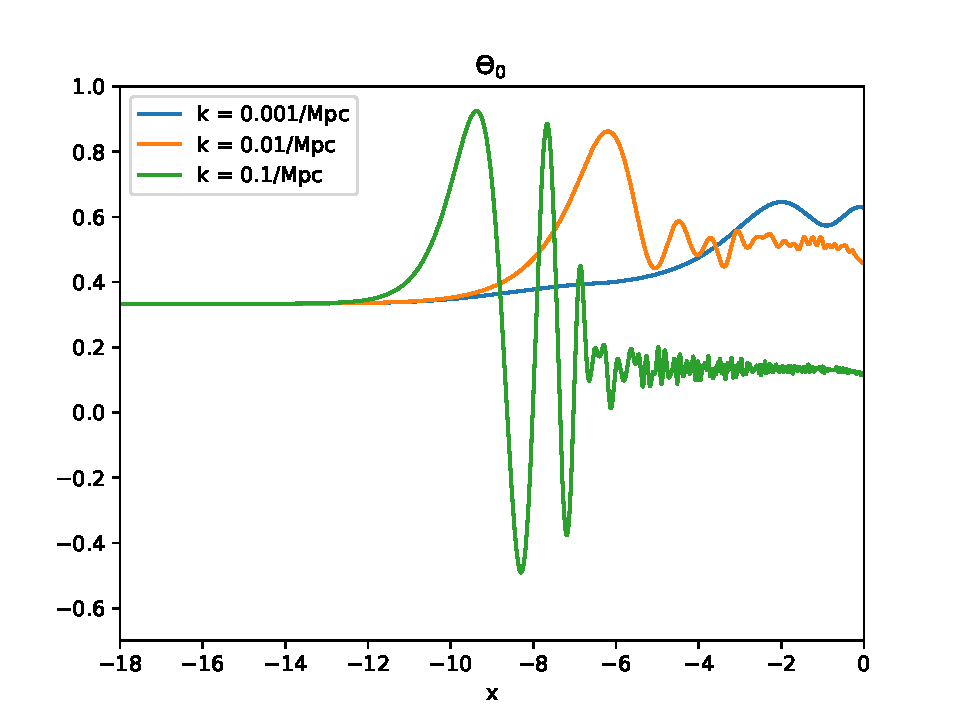
\includegraphics[scale=0.6]{../figures/milestone3/test_theta_0.pdf}
   \caption{The photon temperature monopole, $\Theta_0$, at different scales, $k$.}\label{fig:test3}
\end{figure}

\begin{figure}[h!]
   %\hspace{-0.48cm}   
   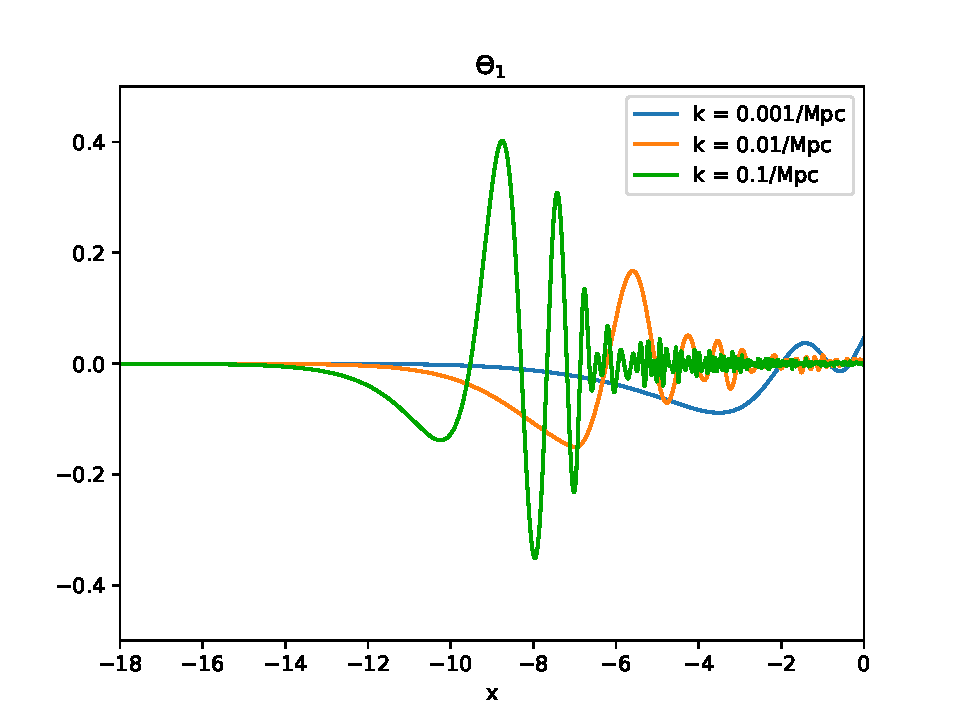
\includegraphics[scale=0.6]{../figures/milestone3/test_theta_1.pdf}
   \caption{The photon temperature dipole, $\Theta_1$, at different scales, $k$.}\label{fig:test4}
\end{figure}

\begin{figure}[h!]
   %\hspace{-0.48cm}   
   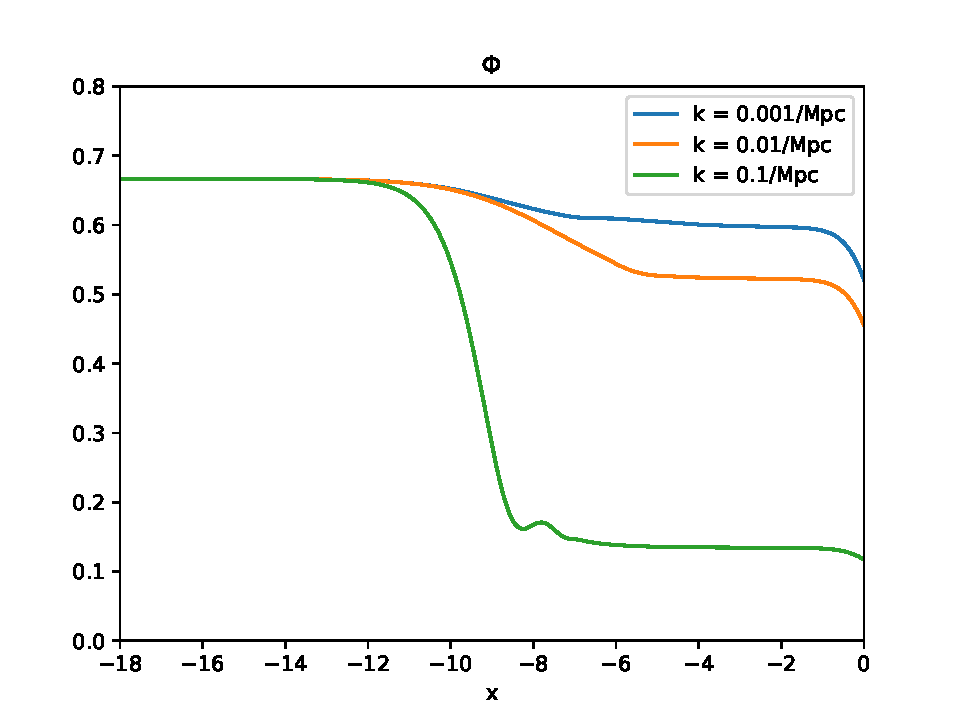
\includegraphics[scale=0.6]{../figures/milestone3/test_phi.pdf}
   \caption{The gravitational potential, $\Phi$, at different scales, $k$.}\label{fig:test5}
\end{figure}

\subsubsection{Results}
%theory section maybe???
% write about the slope of delta_cdm and compare to analytical result...all plots in general
For our results we have again used the fiducial cosmology parameters of \cite{winther:2023}, but we removed the neutrinos from the background.
Since we do not perturb the neutrinos, we believe including them in the background would be inconsistent. We also noted that the results we got with neutrinos included
did not agree with CMB observations.\\
\\
In figure \ref{fig:delta_cdm_delta_b_zoom}, which is a zoomed in version of figure \ref{fig:delta_cdm_delta_b}, we see more clearly what is going on. Gravity travels with the same speed as light. This means that the conformal time, $\eta$,
gives us the maximum reach of gravity at any given time. Therefore, if the scale, $k$, of interest is larger than the conformal time, we should not see any correlation,
since the scale is causally disconnected. Using that Fourier modes enter the particle horizon when $k\eta=1$, we find
that the scale $k=10/\mathrm{Mpc}$ enters the particle horizon at $x\sim -15.4$.
We see that our results are consistent with the theory, as CDM clusters on this scale at $x\sim -16$. The reason why the baryonic overdensity oscillates, is because 
the mass is first compressed by gravity, then the radiation pressure increases such that the mass rebounds, as seen in figure \ref{fig:delta_cdm_delta_b_delta_gamma}. This process is then repeated until the Jeans mass is reached, where the Jeans mass is the mass needed to form structure.
Since the Jeans mass, in a static universe, depends linearly on the sound speed, we do not expect baryon structure to form in general before recombination, where the sound speed was $\sim c$, \cite{Shen:2022}. However, right after recombination  
the sound speed freezes out, i.e. the photons pressure is released, and structures can more easily form. As recombination happened at $x\sim -7$, we can see in our results that the baryon overdensity starts to continously increase at this time for scales that have entered the horizon.
For CDM we do not have any oscillating behavior at early times since CDM is pressureless and gravity only has to works against the cosmic acceleration.   
We note that the overdensity at some times is less than -1, which by definition is impossible in real space. This is not a concern, since the quantities are in Fourier space, and they have not been scaled to represent physical values. 
\\ \\
In figure \ref{fig:v_cdm_v_b} we see that the oscillations in the baryonic overdensity has an expected corresponding oscillation in the baryonic fluid velocity, as the mass is contracting and rebounding repeatedly.
At a larger scale, seen in green, the mode enters the particle horizon later, and the baryonic overdensity undergoes fewer oscillation. For even larger scales, seen in 
red and blue, the modes enter the particle horizon after recombination and there are no oscillations as expected.\\
\\
In figure \ref{fig:delta_gamma} we see how the temperature overdensity behaves for different scales. The corresponding oscillations in the photon fluid velocity can be seen in figure \ref{fig:v_gamma}.
At early times, the photons interact strongly with the baryons, such that they equilibrize. This is clearly seen in figure \ref{fig:delta_cdm_delta_b_delta_gamma}. After 
recombination, the photons will no longer follow the evolution of the baryons. This is because the baryons cluster more and more due to gravity, while photons
do not. We see from the orange graph in \ref{fig:delta_gamma} that the temperature overdensity increases as the scale enters
the horizon and the evolution follows that of the baryons. However, at recombination, the pressure is released, so the temperature does not increase again with the baryons
as we observe for smaller scales that enter the horizon at earlier times. Since the orange graph, with $k = 0.01/Mpc$ is large at recombination, we expect there to be strong
correlation in the CMB power spectrum at these comoving scales, since it is the photons released at recombination we observe today. We note that the photon overdensity in the blue graph, with $k = 0.001/Mpc$
which enters the horizon later, also increases with the baryon overdensity even after recombination when the photons have decoupled from the baryons. This may suggest that
there are still some interactions between the photons and the baryons. Another explanation is seen from figures \ref{fig:phi} and \ref{fig:phi_psi} where the gravitational potentials are plotted.
We see that for large scales at late times, the potentials are at their largest value. This may explain why the photons cluster even after recombination, since general relativity predicts that 
light is affected by the gravitational potential.\\
\\
The evolution of the gravitational potential in \ref{phi} is clearly dependent on when the scale crosses the horizon, and if the crossing happens in the radiation 
era or in the matter era. In the radiation era, the photon perturbations will be the dominant quantity that can affect the potential. 
Since the photon perturbations do not grow in time, the potential will be washed out due to the expansion of the universe.
This is clearly observed in the plot, as the scales that enter in the radiation era starts to decrease as they cross the horizon. For the scales that enter in 
the matter era, the evolution is quite different. Inside the matter era, the dominant quantity to affect the potential is the matter perturbations. We know that the matter
perturbations grow in the matter era, and it can be shown analytically that the potential will be constant, but it takes some time before the universe becomes
matter dominated after radiation-matter equality. We note that the $k = 0.001/Mpc$ scale is the only scale where $\Phi$
decreases before it enters the horizon. 
The fact that the potential changes before horizon crossing is unexpected, and should be explored in future studies.
At very late times, the potential decreases again due to dark energy,
which washes out the potential through more rapid expansion.\\
\\
In figure \ref{fig:phi_psi} we see that the sum of the potentials are large for large scales at late times. The potential $\Phi$ in the Newtonian gauge can be related 
to the Newtonian gravitational potential. We see that during the matter era, there is a strong potential at large scales.\\
\\
In figure \ref{fig:theta2} we see the photon quadrupole, which is analogous to a higher order Taylor expansion term. This term will therefore tell us about the 
finer structure of the photon temperature fluctuations. Since the observed CMB is a measurement of the photon temperature fluctuations that originate
from the universe at recombination, $x \sim -7$, we can expect there to be correlation at scales corresponding to $k = 0.1/Mpc$. The larger scale, $k = 0.001/Mpc$, 
is very small and flat at this time, so we should not expect to see correlations at these scales.    


%Show and discuss the results.

\begin{figure}[H]
   %\hspace{-0.48cm}   
   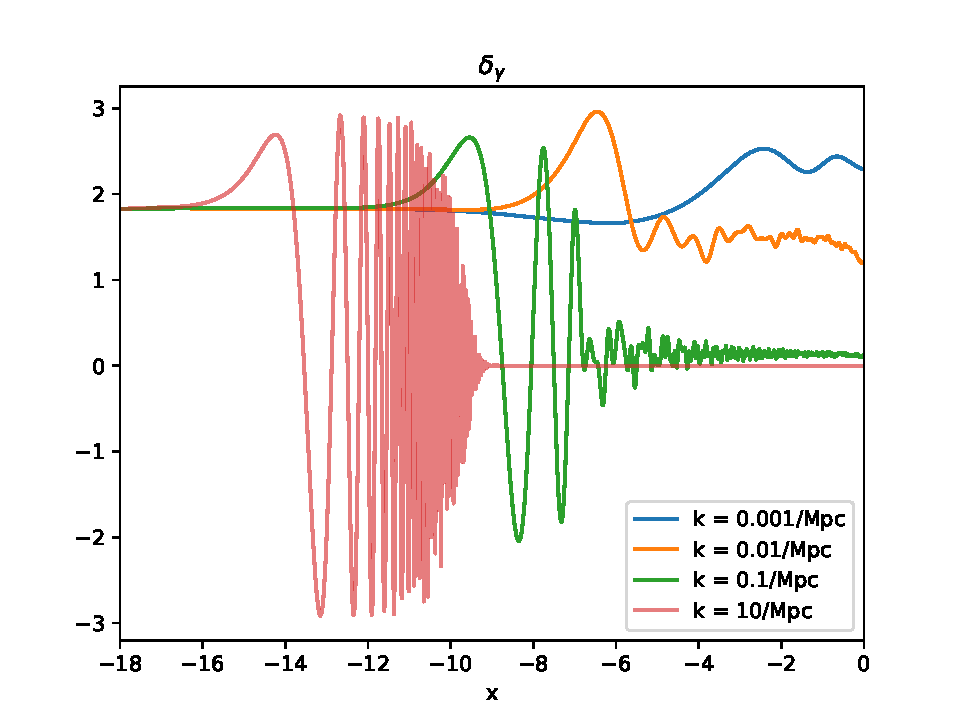
\includegraphics[scale=0.6]{../figures/milestone3/delta_gamma.pdf}
   \caption{The comparable photon overdensity, $\delta_\gamma = 4\Theta_0$, at four different scales, $k$. }\label{fig:delta_gamma}
\end{figure}

\begin{figure}[H]
   %\hspace{-0.48cm}   
   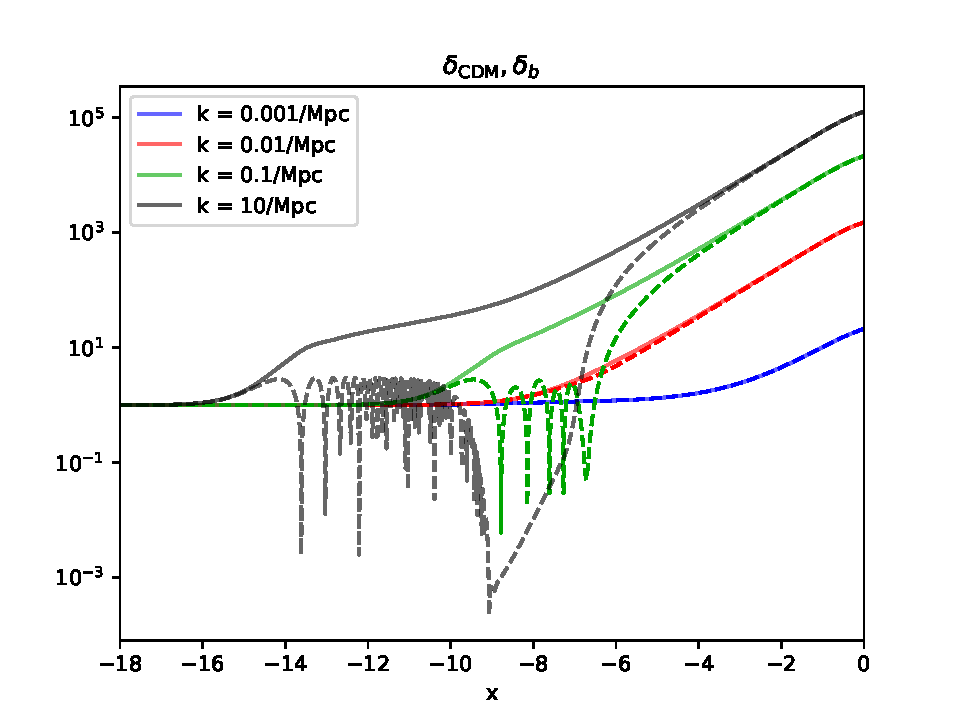
\includegraphics[scale=0.6]{../figures/milestone3/delta_cdm_delta_b.pdf}
   \caption{The CDM overdensity and the absolute value of the baryon overdensity plotted at four different scales, $k$. The solid lines are for CDM and the dotted lines are for baryons.}\label{fig:delta_cdm_delta_b}
\end{figure}

\begin{figure}[H]
   %\hspace{-0.48cm}   
   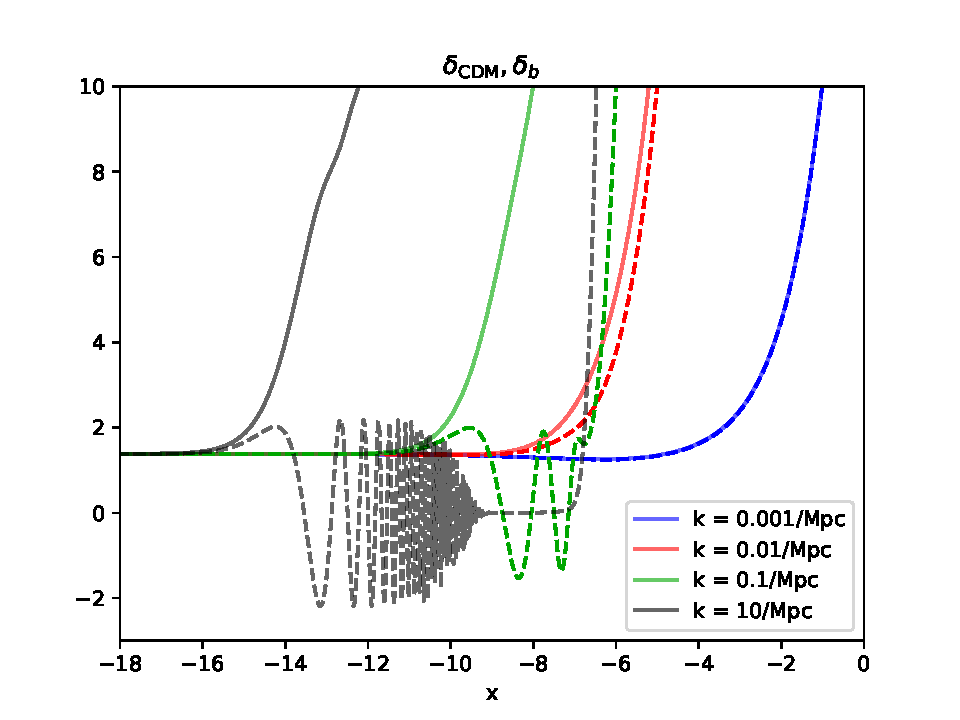
\includegraphics[scale=0.65]{../figures/milestone3/delta_cdm_delta_b_zoom.pdf}
   \caption{A closer look at figure \ref{fig:delta_cdm_delta_b} with linear y-scale and with the correct sign for the baryon overdensity.}\label{fig:delta_cdm_delta_b_zoom}
\end{figure}

\begin{figure}[H]
   %\hspace{-0.48cm}   
   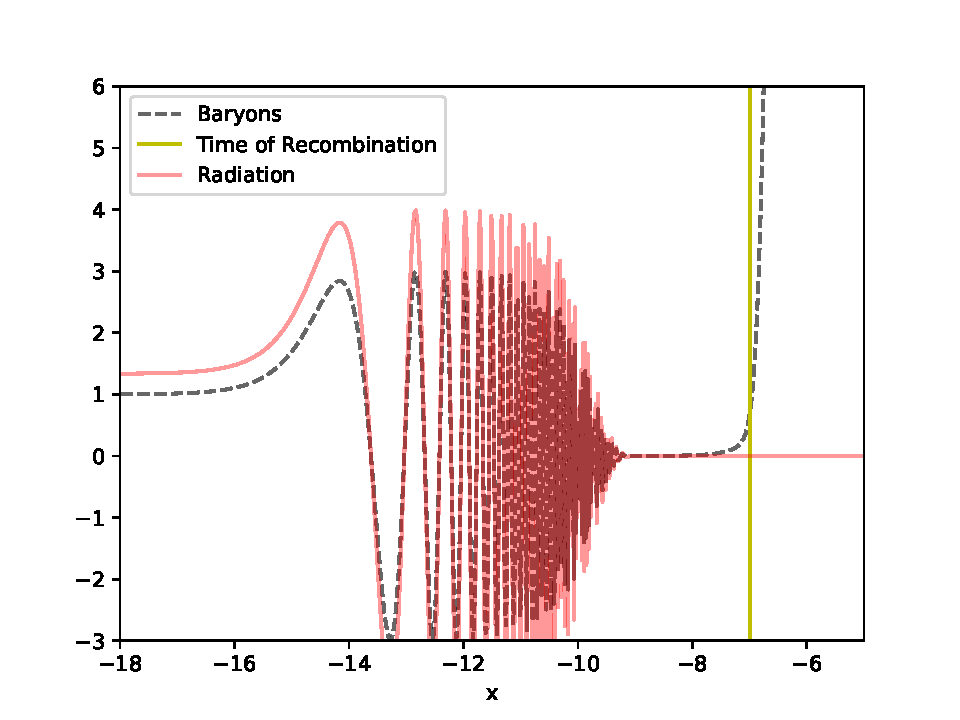
\includegraphics[scale=0.65]{../figures/milestone3/delta_cdm_delta_b_delta_gamma.pdf}
   \caption{Same as figure \ref{fig:delta_cdm_delta_b_zoom} at $k=10/Mpc$ with radiation overdensity included.}\label{fig:delta_cdm_delta_b_delta_gamma}
\end{figure}

\begin{figure}[H]
   %\hspace{-0.48cm}   
   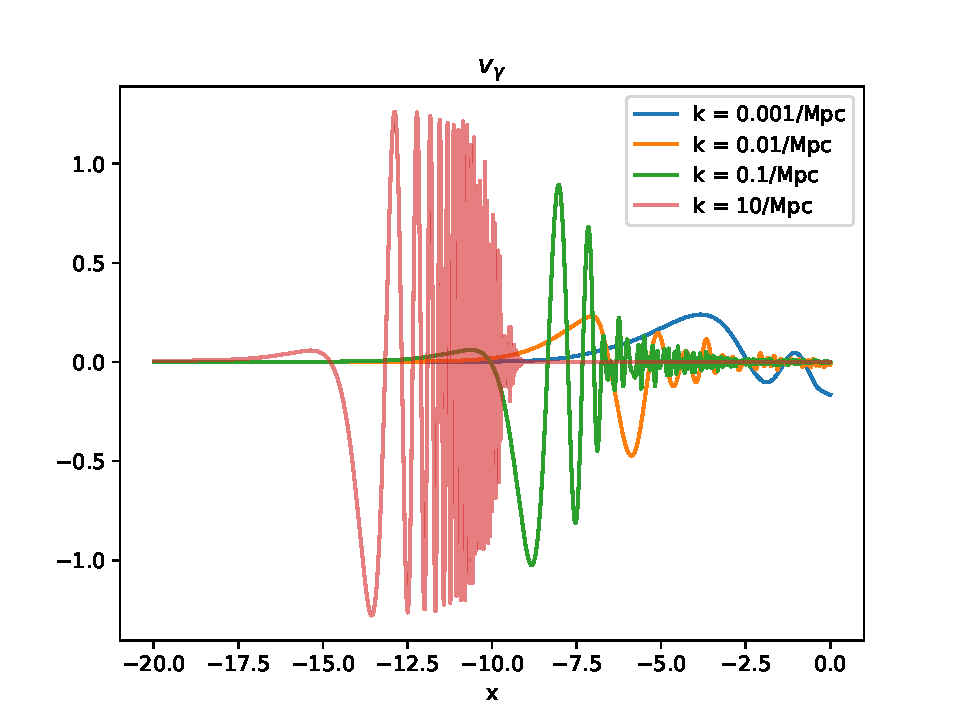
\includegraphics[scale=0.6]{../figures/milestone3/v_gamma.pdf}
   \caption{The photon velocity perturbation, $v_\gamma=-3\Theta_1$, at four different scales, $k$.}\label{fig:v_gamma}
\end{figure}

\begin{figure}[H]
   %\hspace{-0.48cm}   
   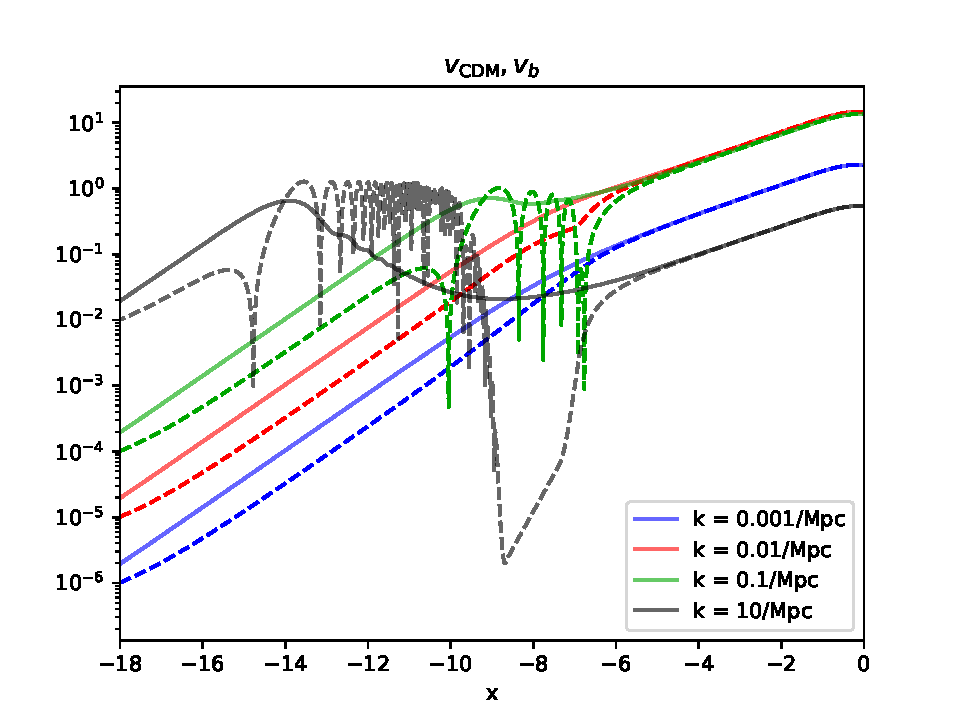
\includegraphics[scale=0.6]{../figures/milestone3/v_cdm_v_b.pdf}
   \caption{The CDM velocities, in solid lines, and the absolute value of the baryon velocities,
   in dotted lines, are plotted at four different scales, $k$.}\label{fig:v_cdm_v_b}
\end{figure}

\begin{figure}[H]
   %\hspace{-0.48cm}   
   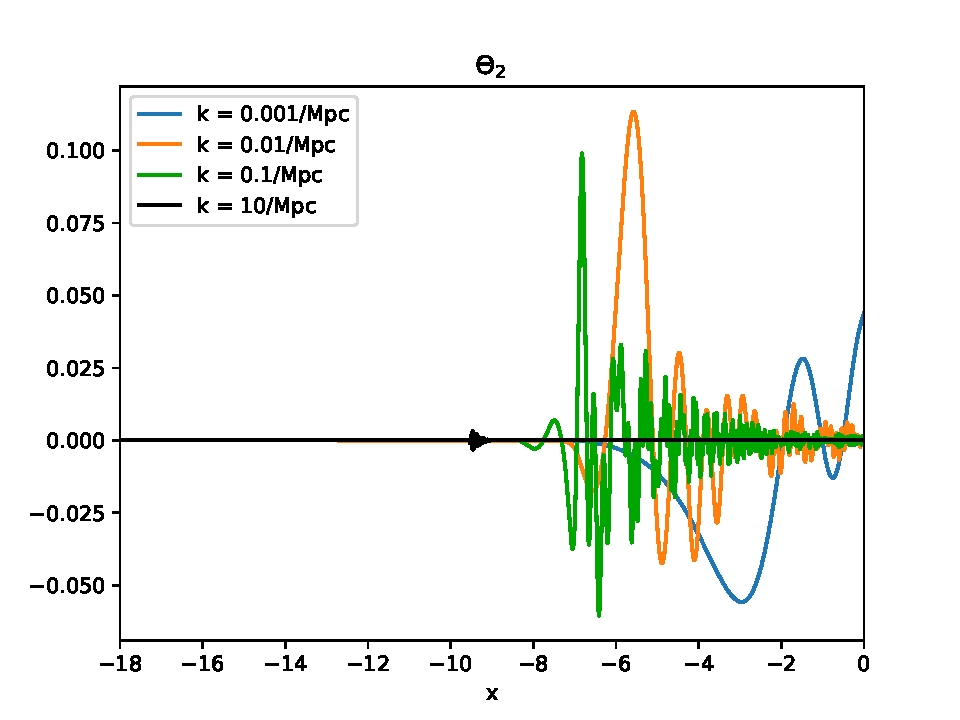
\includegraphics[scale=0.65]{../figures/milestone3/theta_2.pdf}
   \caption{The photon temperature quadrupole, $\Theta_2$, at four different scales, $k$.}\label{fig:theta2}
\end{figure}

\begin{figure}[H]
   %\hspace{-0.48cm}   
   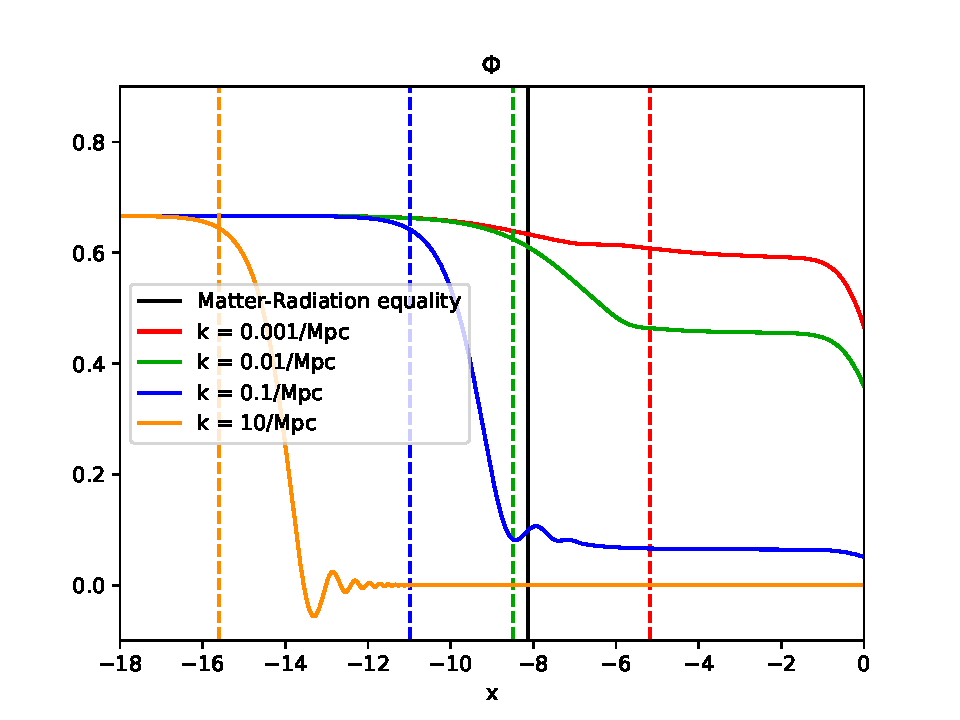
\includegraphics[scale=0.6]{../figures/milestone3/phi.pdf}
   \caption{The gravitational potential at four different scales, $k$. The dotted line denotes the time of horizon crossing for the scale with the same color.}\label{fig:phi}
\end{figure}

\begin{figure}[H]
   %\hspace{-0.48cm}   
   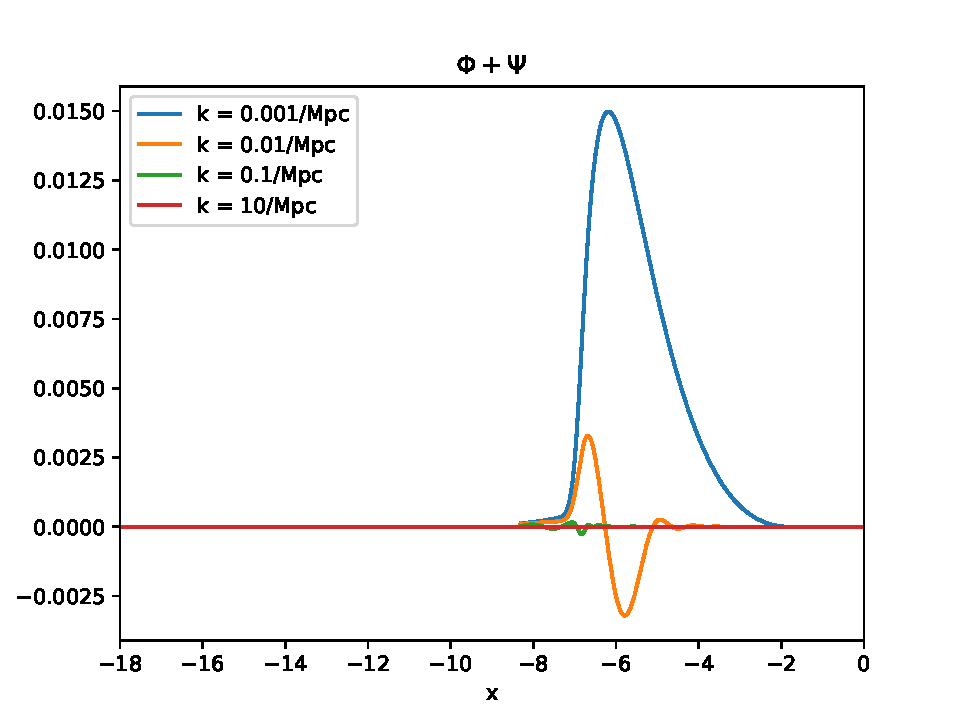
\includegraphics[scale=0.6]{../figures/milestone3/phi_psi.pdf}
   \caption{The sum of the two gravitational potentials, $\Phi$ and $\Psi$, at four different scales, $k$.}\label{fig:phi_psi}
\end{figure}



\section{Milestone IV}
%for milestone 3 we turn of neutrinos, as they may lead to inconsistencies
%Some introduction about what it is all about.

\subsection{Theory}
%The theory behind this milestone.
The CMB power spectrum, $C_\ell$, is defined as 
\begin{equation}
   C_\ell \equiv \langle |a_{\ell m}|^2 \rangle = \langle a_{\ell m}a_{\ell m}^* \rangle,
\end{equation}
where $a_{lm}$ are the coefficients of the spherical harmonics used to transform the CMB temperature field. In principle, it is possible to get the $C_\ell$s by evaluating $\Theta_\ell(k,x=0)$
and Fourier transform the coefficients back to real space, \cite{winther:2023}. However, as we are interested in $\ell$ values from $\sim 10^0$ to $\sim 10^3$, this approach would 
be very slow since we would have to solve thousands of coupled differential equations in the previous milestone. Instead, we can use the line of sight integral given below to calculate $\Theta_\ell(x=0,k)$ for arbitrary $\ell$.
\begin{equation}
   \Theta_\ell(k, x=0) = \int_{-\infty}^{0} \tilde{S}(k,x) j_\ell[k(\eta_0-\eta)] dx,
\end{equation}
where the source function is defined as 

\begin{equation}
   \begin{aligned}
   \tilde{S}(k,x) &= \tilde{g}\left[ \Theta_0 + \Psi + \frac{1}{4}\Pi\right] + e^{-\tau} \left[\Psi^\prime-\Phi^\prime\right] \\
   &-\frac{1}{ck}\frac{d}{dx}(\mathcal{H}\tilde{g}v_b) + \frac{3}{4c^2k^2} \frac{d}{dx}
   \left[\mathcal{H}\frac{d}{dx} (\mathcal{H}\tilde{g}\Theta_2)\right]. 
   \end{aligned}
\end{equation}
$j_\ell(y)$ is the spherical Bessel function.\\
\\
The CMB power spectrum can now be expressed as 
   \begin{equation}
      C_\ell = \frac{2}{\pi}\int k^2P_{\rm primordial}(k) \Theta_\ell^2(k)dk,
   \end{equation}
which can be written as 
\begin{equation}\label{eq:m4_cell}
   C_\ell = 4\pi \int_0^{\infty} A_s \left(\frac{k}{k_{\rm pivot}}\right)^{n_s-1} \Theta_\ell^2(k) \frac{dk}{k}
\end{equation}
by using a Harrison-Zel'dovich primordial power spectrum \cite{winther:2023}.\\
\\
The matter power spectrum is defined by
\begin{equation}
   P(k,x) = |\Delta_M(k,x)|^2P_{\rm primordial}(k),
\end{equation}
where $\Delta_M(k,x) \equiv \frac{c^2k^2\Phi(k,x)}{\frac{3}{2}\Omega_{M 0} a^{-1} H_0^2}$.
\subsection{Implementation details}
%bessel slpline did not work
%used trapezoid for the integrals
Something about the numerical work.

\subsection{Results}

\subsubsection{Test results}
In figures \ref{fig:m4_matter_test} and \ref{fig:m4_cell_test} we have plotted the plots shown in \cite{winther:2023} under "testing your code". We see that the CMB power
spectrum has the same shape, but the values are too large. The same can be said about the matter power spectrum. This suggests that our results will in general be too large.
There can be many reasons for this discrepancy, but we believe the error comes either from the calculation of the source function, or from an early $k$ cut-off for the $C_\ell$ integration as we will discuss later.

\begin{figure}[H]
   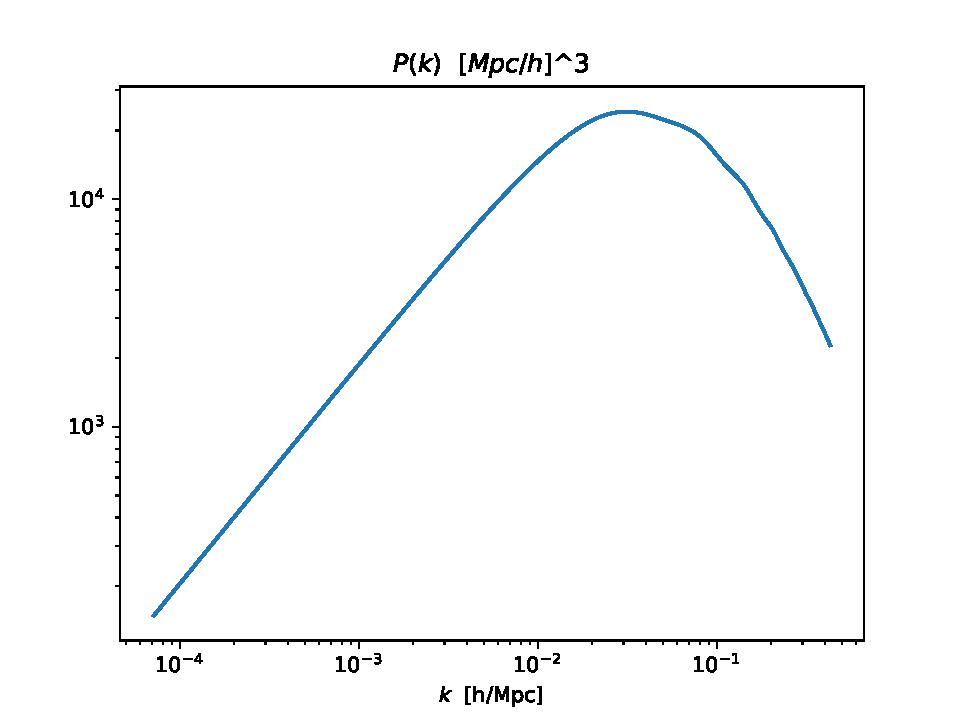
\includegraphics[scale=0.6]{../figures/milestone4/matter_test.pdf}
   \caption{The matter power spectrum with test parameters given by \ref{tab:test_parameters}.}\label{fig:m4_matter_test}
\end{figure}

\begin{figure}[H]
   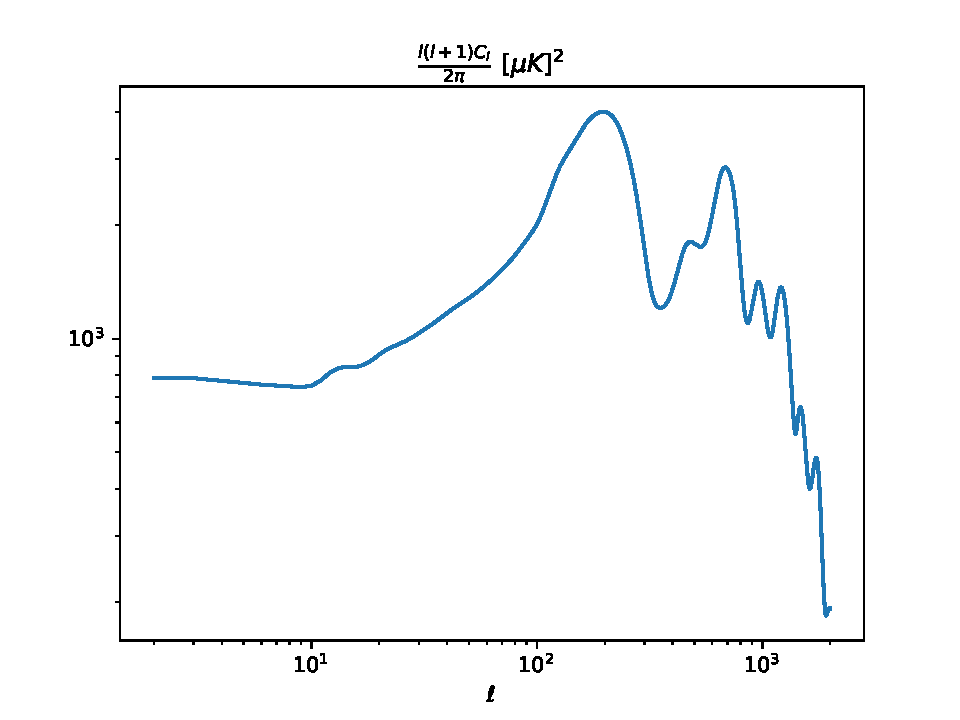
\includegraphics[scale=0.6]{../figures/milestone4/cell_test.pdf}
   \caption{The CMB power spectrum with test parameters given by \ref{tab:test_parameters}.}\label{fig:m4_cell_test}
\end{figure}



\subsubsection{Our results}
In figures \ref{fig:m4_theta2},\ref{fig:m4_theta10},\ref{fig:m4_theta100} and \ref{fig:m4_theta1200} we see some of the photon multipoles $\Theta_\ell(k)$ at $x=0$. 
We clearly see that these functions are oscillating as expected due to the periodic nature of the spherical Bessel functions. The $k$ range in the plot is the range used
in the integral in equation \ref{eq:m4_cell}. We see that the cut-off in the $k$ range seems too early. However, since we only need ${\Theta_\ell}^2$ the problem is not
as serious. This is seen in figures \ref{fig:m4_comparison1} and \ref{fig:m4_comparison2}. The cut-off exists only to reduce computation time.

\begin{figure}[H]
   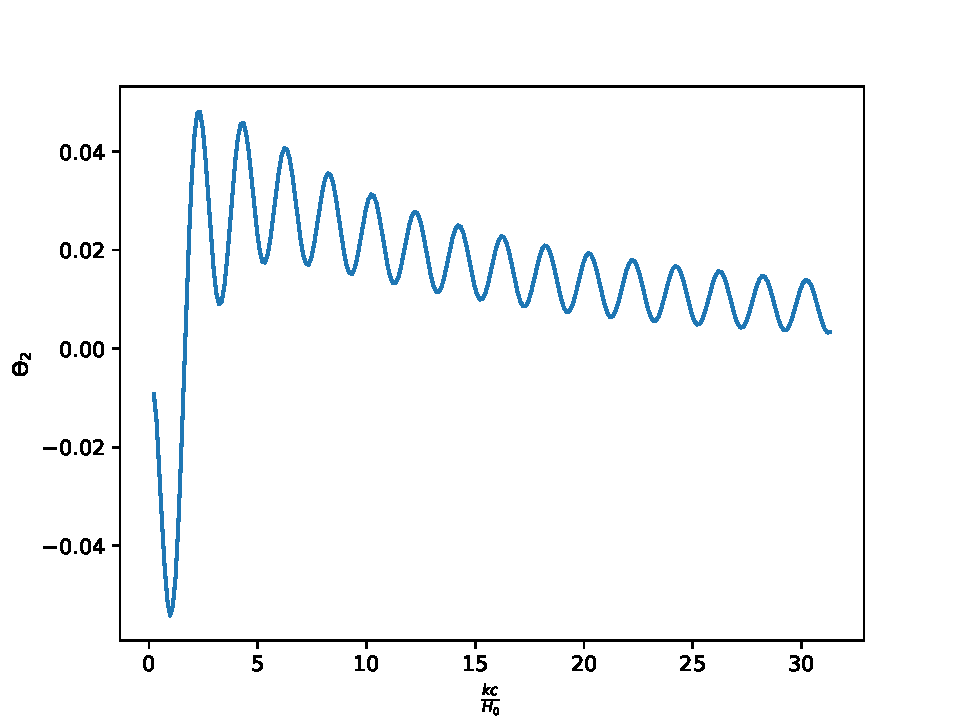
\includegraphics[scale=0.6]{../figures/milestone4/theta_2.pdf}
   \caption{The transfer function, $\Theta_2(k)$.}\label{fig:m4_theta2}
\end{figure}

\begin{figure}[H]
   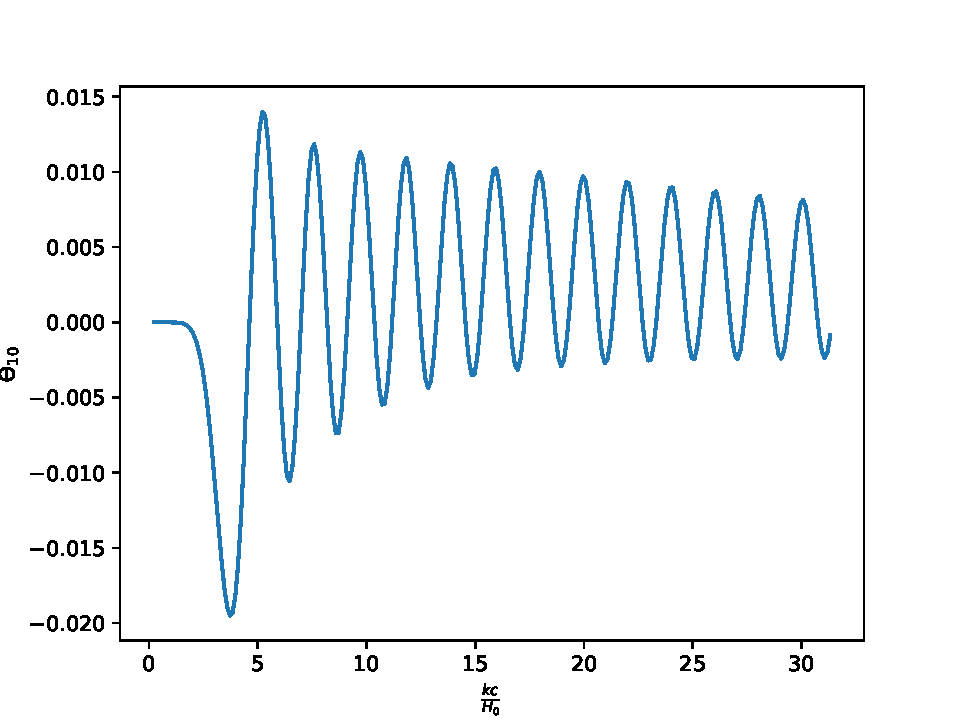
\includegraphics[scale=0.6]{../figures/milestone4/theta_10.pdf}
   \caption{The transfer function, $\Theta_{10}(k)$.}\label{fig:m4_theta10}
\end{figure}

\begin{figure}[H]
   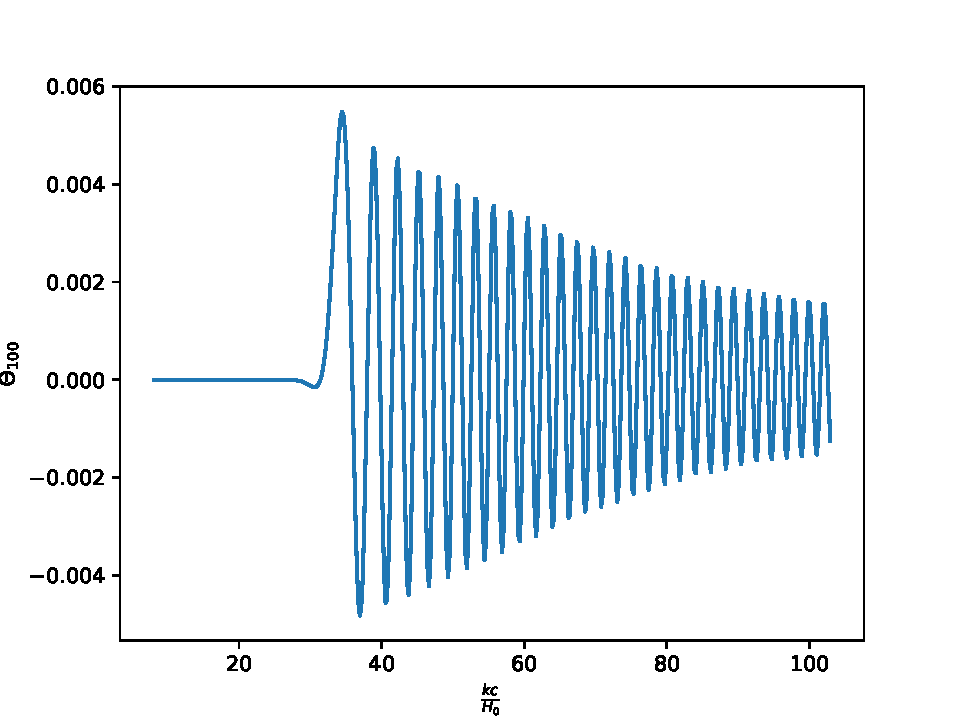
\includegraphics[scale=0.6]{../figures/milestone4/theta_100.pdf}
   \caption{The transfer function, $\Theta_{100}(k)$.}\label{fig:m4_theta100}
\end{figure}

\begin{figure}[H]
   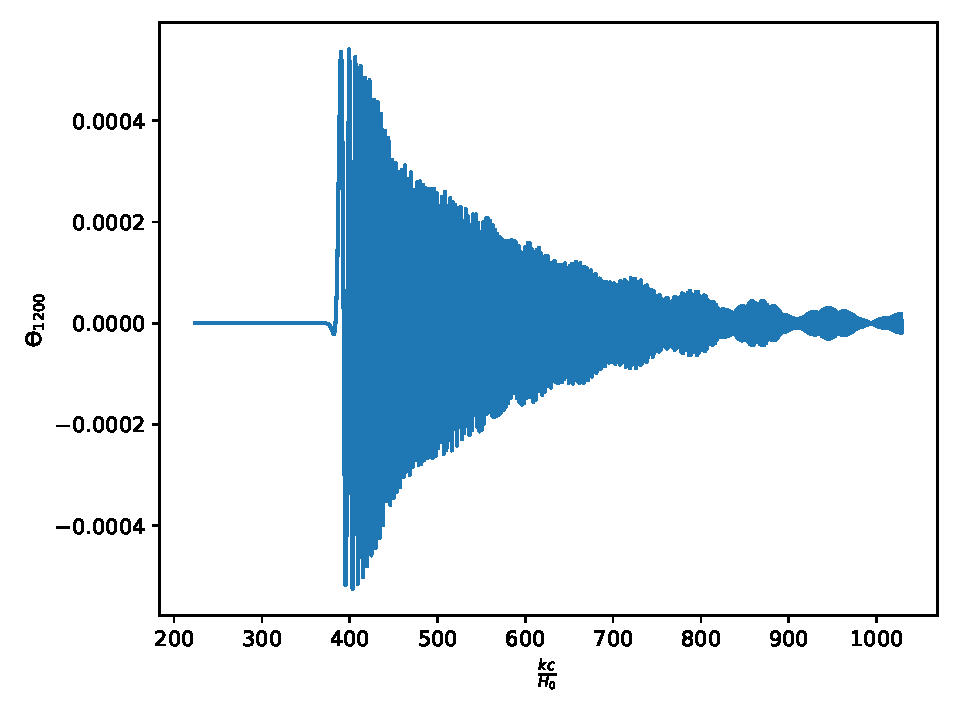
\includegraphics[scale=0.6]{../figures/milestone4/theta_1200.pdf}
   \caption{The transfer function, $\Theta_{1200}(k)$.}\label{fig:m4_theta1200}
\end{figure}

\begin{figure}[H]
   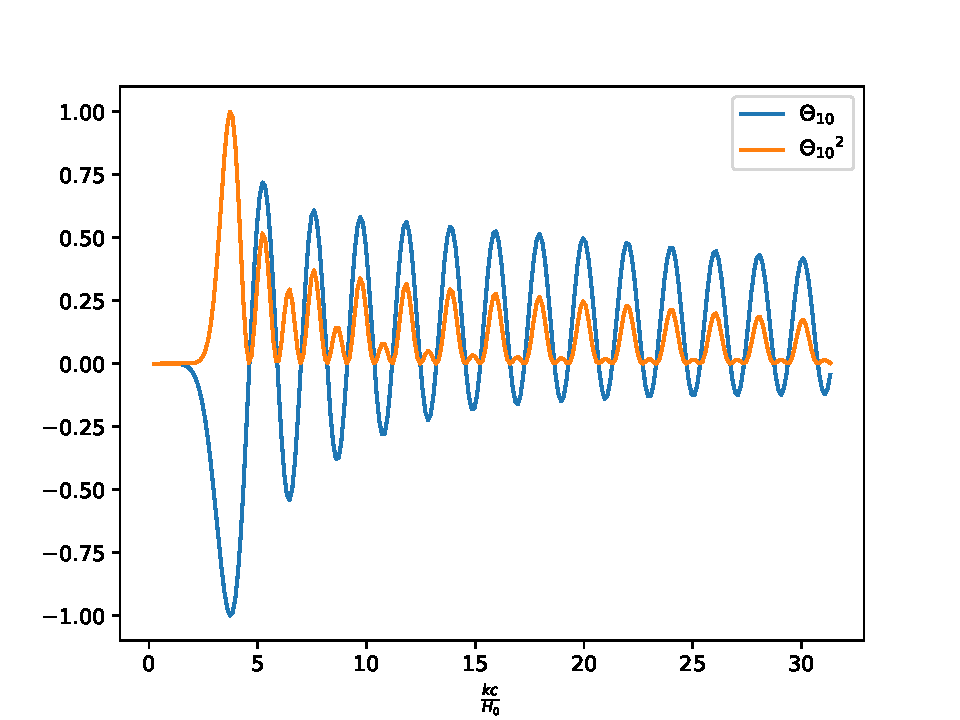
\includegraphics[scale=0.6]{../figures/milestone4/comparison1.pdf}
   \caption{The transfer function, $\Theta_{10}$ and its square both normalized to one.}\label{fig:m4_comparison1}
\end{figure}

\begin{figure}[H]
   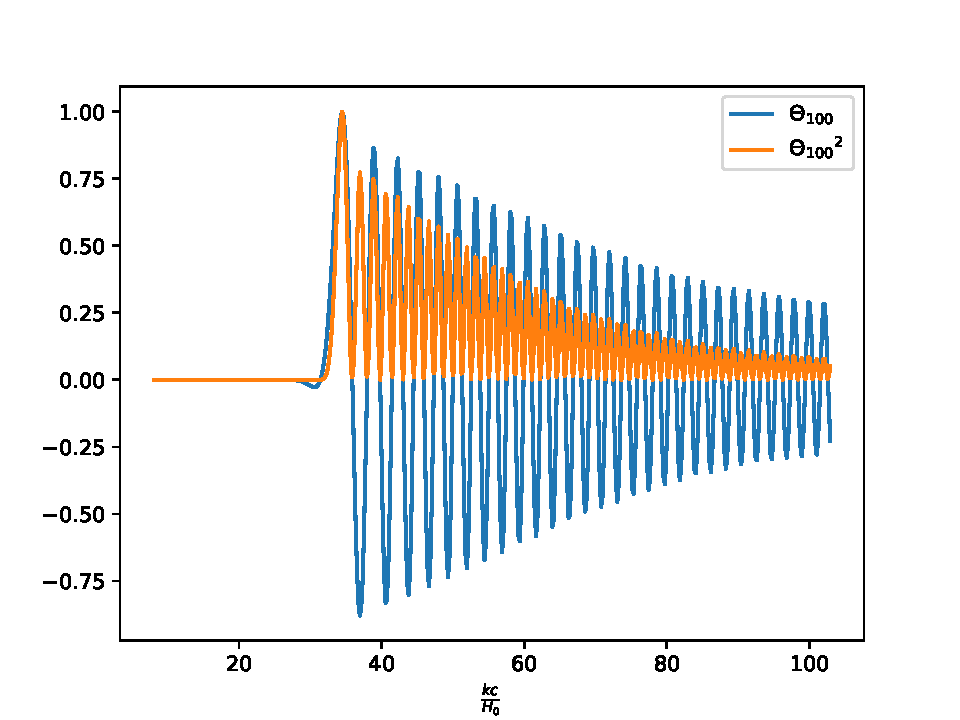
\includegraphics[scale=0.6]{../figures/milestone4/comparison2.pdf}
   \caption{The transfer function, $\Theta_{100}$ and its square both normalized to one.}\label{fig:m4_comparison2}
\end{figure}



\begin{figure}[H]
   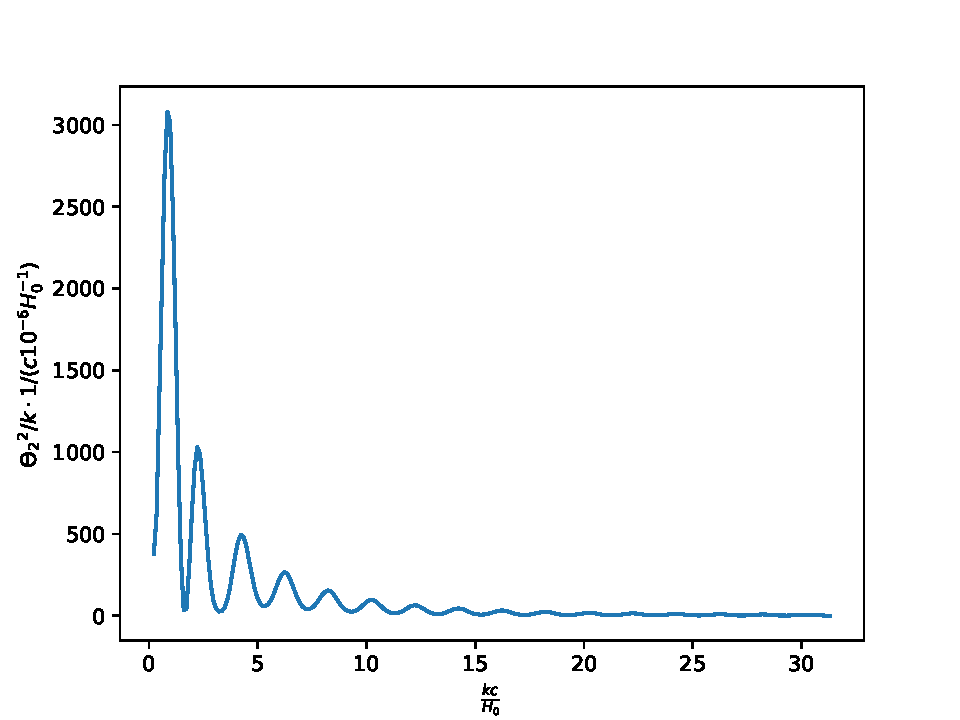
\includegraphics[scale=0.6]{../figures/milestone4/theta_2_squared.pdf}
   \caption{The integrand of the $C_{2}$ integral.}\label{fig:m4_theta2_squared}
\end{figure}

\begin{figure}[H]
   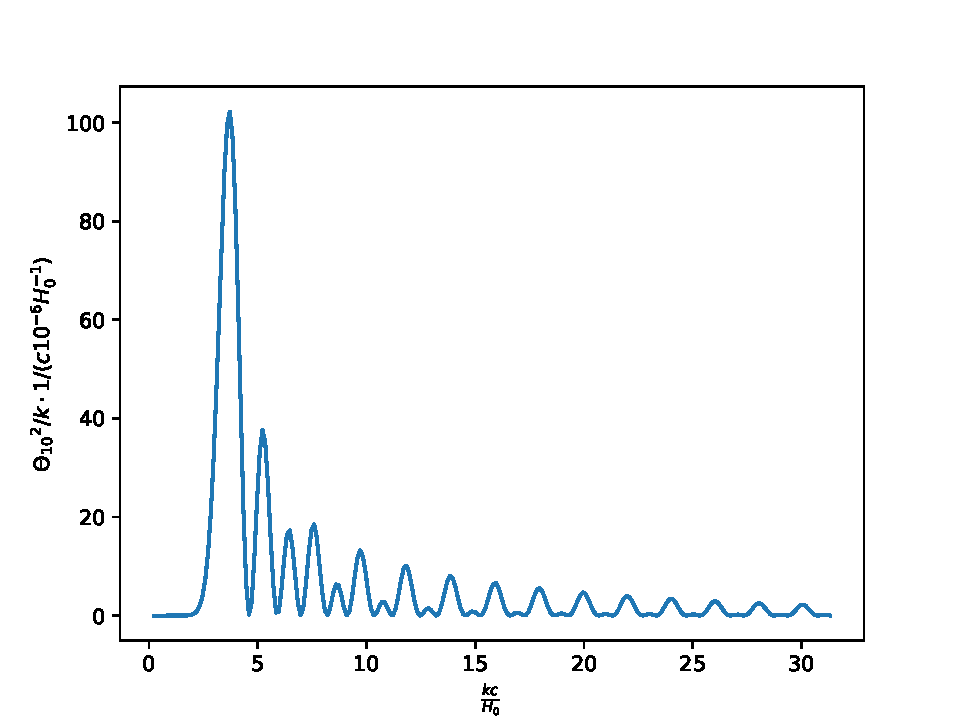
\includegraphics[scale=0.6]{../figures/milestone4/theta_10_squared.pdf}
   \caption{The integrand of the $C_{10}$ integral.}\label{fig:m4_theta10_squared}
\end{figure}

\begin{figure}[H]
   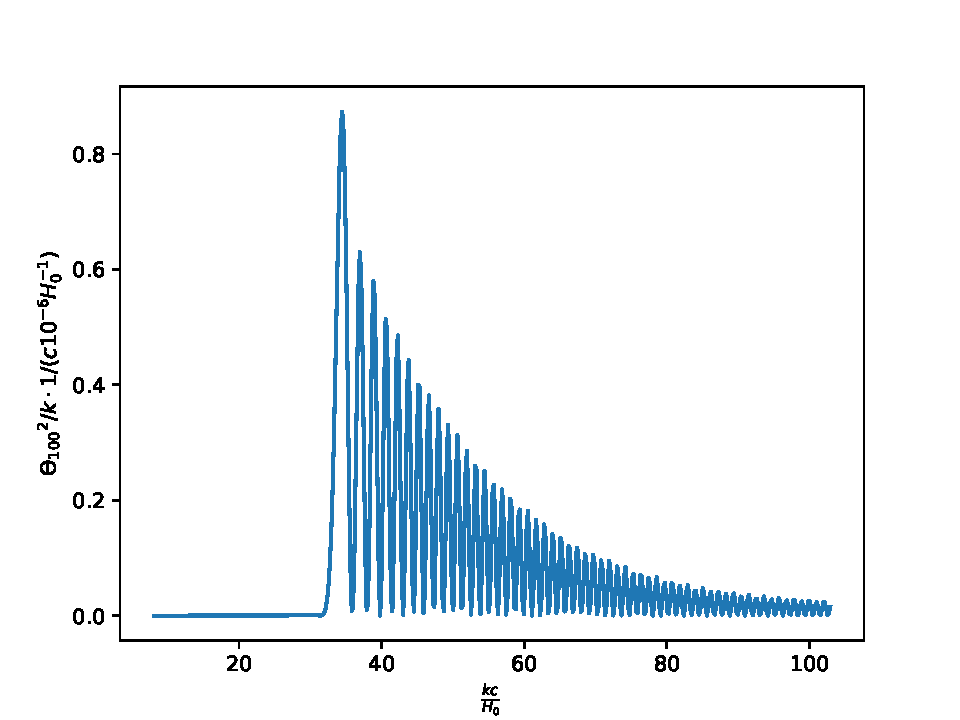
\includegraphics[scale=0.6]{../figures/milestone4/theta_100_squared.pdf}
   \caption{The integrand of the $C_{100}$ integral.}\label{fig:m4_theta100_squared}
\end{figure}

\begin{figure}[H]
   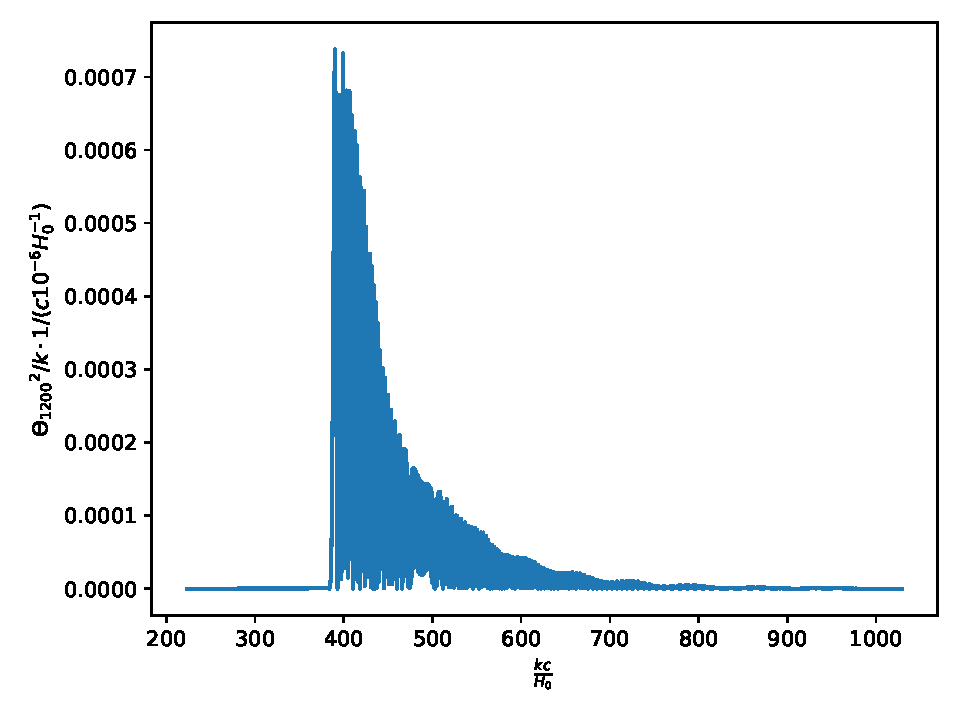
\includegraphics[scale=0.6]{../figures/milestone4/theta_1200_squared.pdf}
   \caption{The integrand of the $C_{1200}$ integral.}\label{fig:m4_theta1200_squared}
\end{figure}





\begin{figure}[H]
   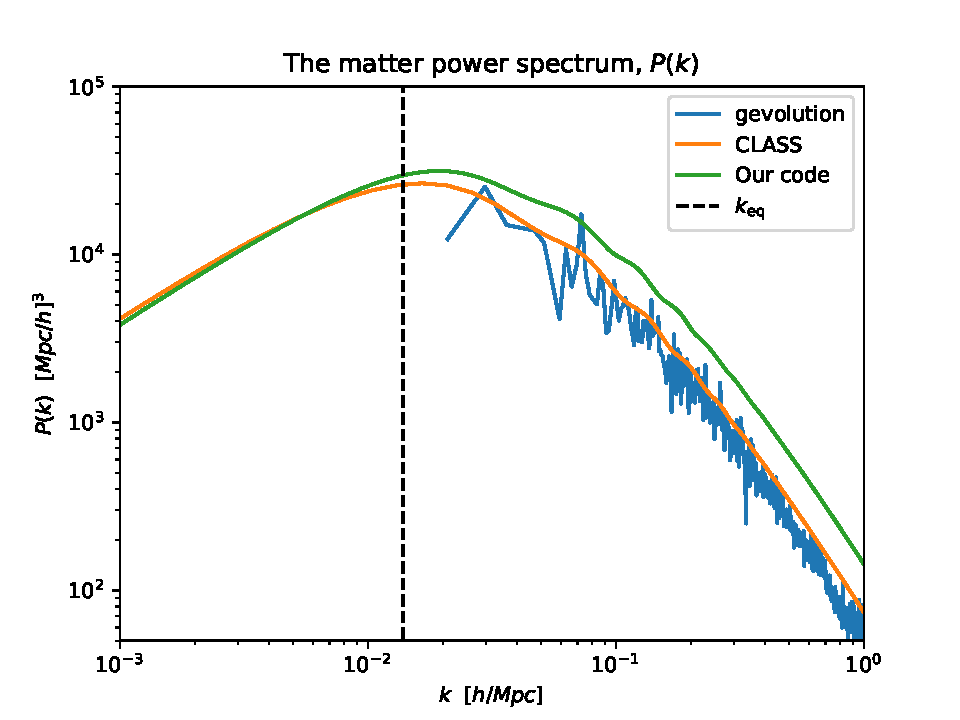
\includegraphics[scale=0.6]{../figures/milestone4/matter_PS.pdf}
   \caption{The matter power spectrum compared to the result of publicly available codes CLASS(Boltzmann) and gevolution(relativistic N-body). CLASS was run with Planck cosmology and gevolution was run for dark matter.}\label{fig:m4_matter_PS}
\end{figure}

\begin{figure}[H]
   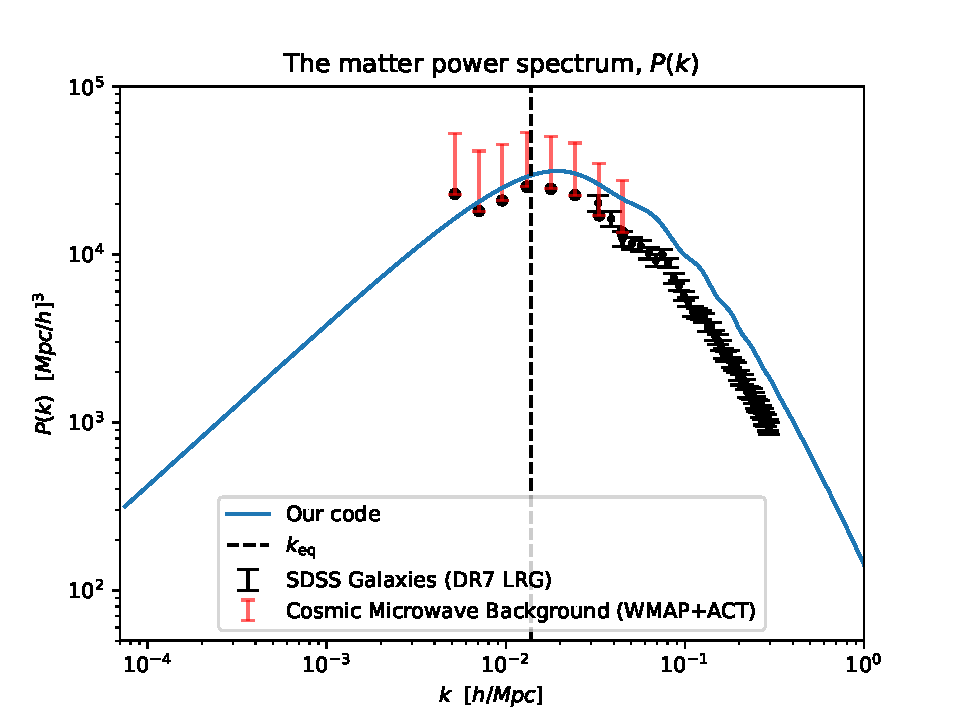
\includegraphics[scale=0.6]{../figures/milestone4/matter_PS_data.pdf}
   \caption{The matter power spectrum with data.}\label{fig:m4_matter_PS_data}
\end{figure}

\begin{figure}[H]
   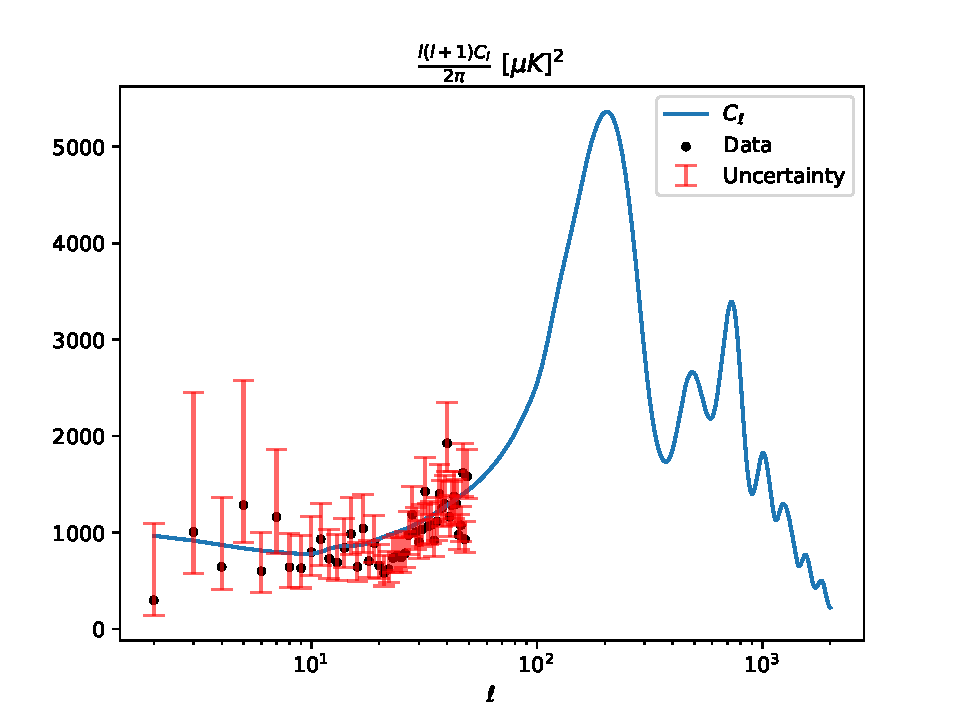
\includegraphics[scale=0.6]{../figures/milestone4/cell.pdf}
   \caption{The CMB power spectrum.}\label{fig:m4_cell}
\end{figure}
\section{Conclusions}

Write a short summary and conclusion in the end. 

%\begin{acknowledgements}
%      I thank my mom for financial support!!!
%\end{acknowledgements}

\bibliographystyle{aa} % style aa.bst
\bibliography{refs} % your references Yourfile.bib
%

%\bibliographystyle{plain} % We choose the "plain" reference style
%\section*{References}
%\bibliography{refs} % Entries are in the refs.bib file

%\begin{thebibliography}{}
%      \bibitem[1966]{baker} Baker, N. 1966,
%      in Stellar Evolution,
%      ed.\ R. F. Stein,\& A. G. W. Cameron
%      (Plenum, New York) 333
%
%      \bibitem[2023]{winther} Winther, H.A. 2023,
%      %\href{https://cmb.wintherscoming.no/milestone1.php}
%\end{thebibliography}

\end{document}